\section{Thực nghiệm và đánh giá}

Các thực nghiệm được thiết kế để trả lời từng câu hỏi riêng biệt. Mọi thực nghiệm dùng cùng tập train/test, cùng 5 fold Stratified và cùng tập chỉ số, chỉ thay đổi một yếu tố tại một thời điểm.

\begin{table}[H]
\centering
\begin{tabular}{c p{6cm} p{6.5cm}}
\toprule
\textbf{Thực nghiệm} & \textbf{Câu hỏi} & \textbf{Cách đánh giá} \\
\midrule
1 & So sánh 4 thuật toán ở cấu hình baseline & 5-fold CV \\
2 & Feature Engineering có cải thiện hiệu năng? & 5-fold CV, so sánh cặp theo fold \\
3 & Class weight hay SMOTE giải quyết mất cân bằng tốt hơn? & 5-fold CV, so sánh cặp theo fold \\
4 & Hyperparameter Tuning cải thiện bao nhiêu? & RandomizedSearchCV trên cùng 5 fold \\
5 & Ngưỡng quyết định nào phù hợp? & Xác suất out-of-fold trên tập train \\
-- & Mô hình cuối cùng và giải thích mô hình & Tập test (dùng một lần) \\
\bottomrule
\end{tabular}
\caption{Tổng quan các thực nghiệm}
\end{table}

So với kế hoạch ban đầu, nhóm không thực hiện thực nghiệm so sánh các phương pháp Encoding/Scaling; mọi thực nghiệm dùng chung One-Hot Encoding và \texttt{StandardScaler} (chỉ cho Logistic Regression).

% ============================================================
\subsection{Experiment 1: So sánh các mô hình baseline}
% ============================================================

\subsubsection{Kết quả cross-validation}

\begin{table}[H]
\centering
\small
\begin{tabular}{lccccc}
\toprule
\textbf{Mô hình} & \textbf{Accuracy} & \textbf{Precision} & \textbf{Recall} & \textbf{F1} & \textbf{ROC-AUC} \\
\midrule
Logistic Regression & \textbf{0,8019} $\pm$ 0,0133 & \textbf{0,6524} $\pm$ 0,0294 & \textbf{0,5431} $\pm$ 0,0460 & \textbf{0,5921} $\pm$ 0,0334 & \textbf{0,8461} $\pm$ 0,0140 \\
XGBoost             & 0,7982 $\pm$ 0,0088 & 0,6501 $\pm$ 0,0255 & 0,5204 $\pm$ 0,0235 & 0,5777 $\pm$ 0,0183 & 0,8413 $\pm$ 0,0084 \\
Random Forest       & 0,7863 $\pm$ 0,0092 & 0,6276 $\pm$ 0,0261 & 0,4803 $\pm$ 0,0215 & 0,5439 $\pm$ 0,0193 & 0,8199 $\pm$ 0,0114 \\
Decision Tree       & 0,7286 $\pm$ 0,0060 & 0,4890 $\pm$ 0,0108 & 0,4957 $\pm$ 0,0141 & 0,4922 $\pm$ 0,0082 & 0,6543 $\pm$ 0,0057 \\
\bottomrule
\end{tabular}
\caption{Kết quả validation của 4 mô hình baseline (Stratified 5-fold CV trên tập train, 19 đặc trưng gốc)}
\label{tab:baseline_cv}
\end{table}

\begin{figure}[H]
\centering
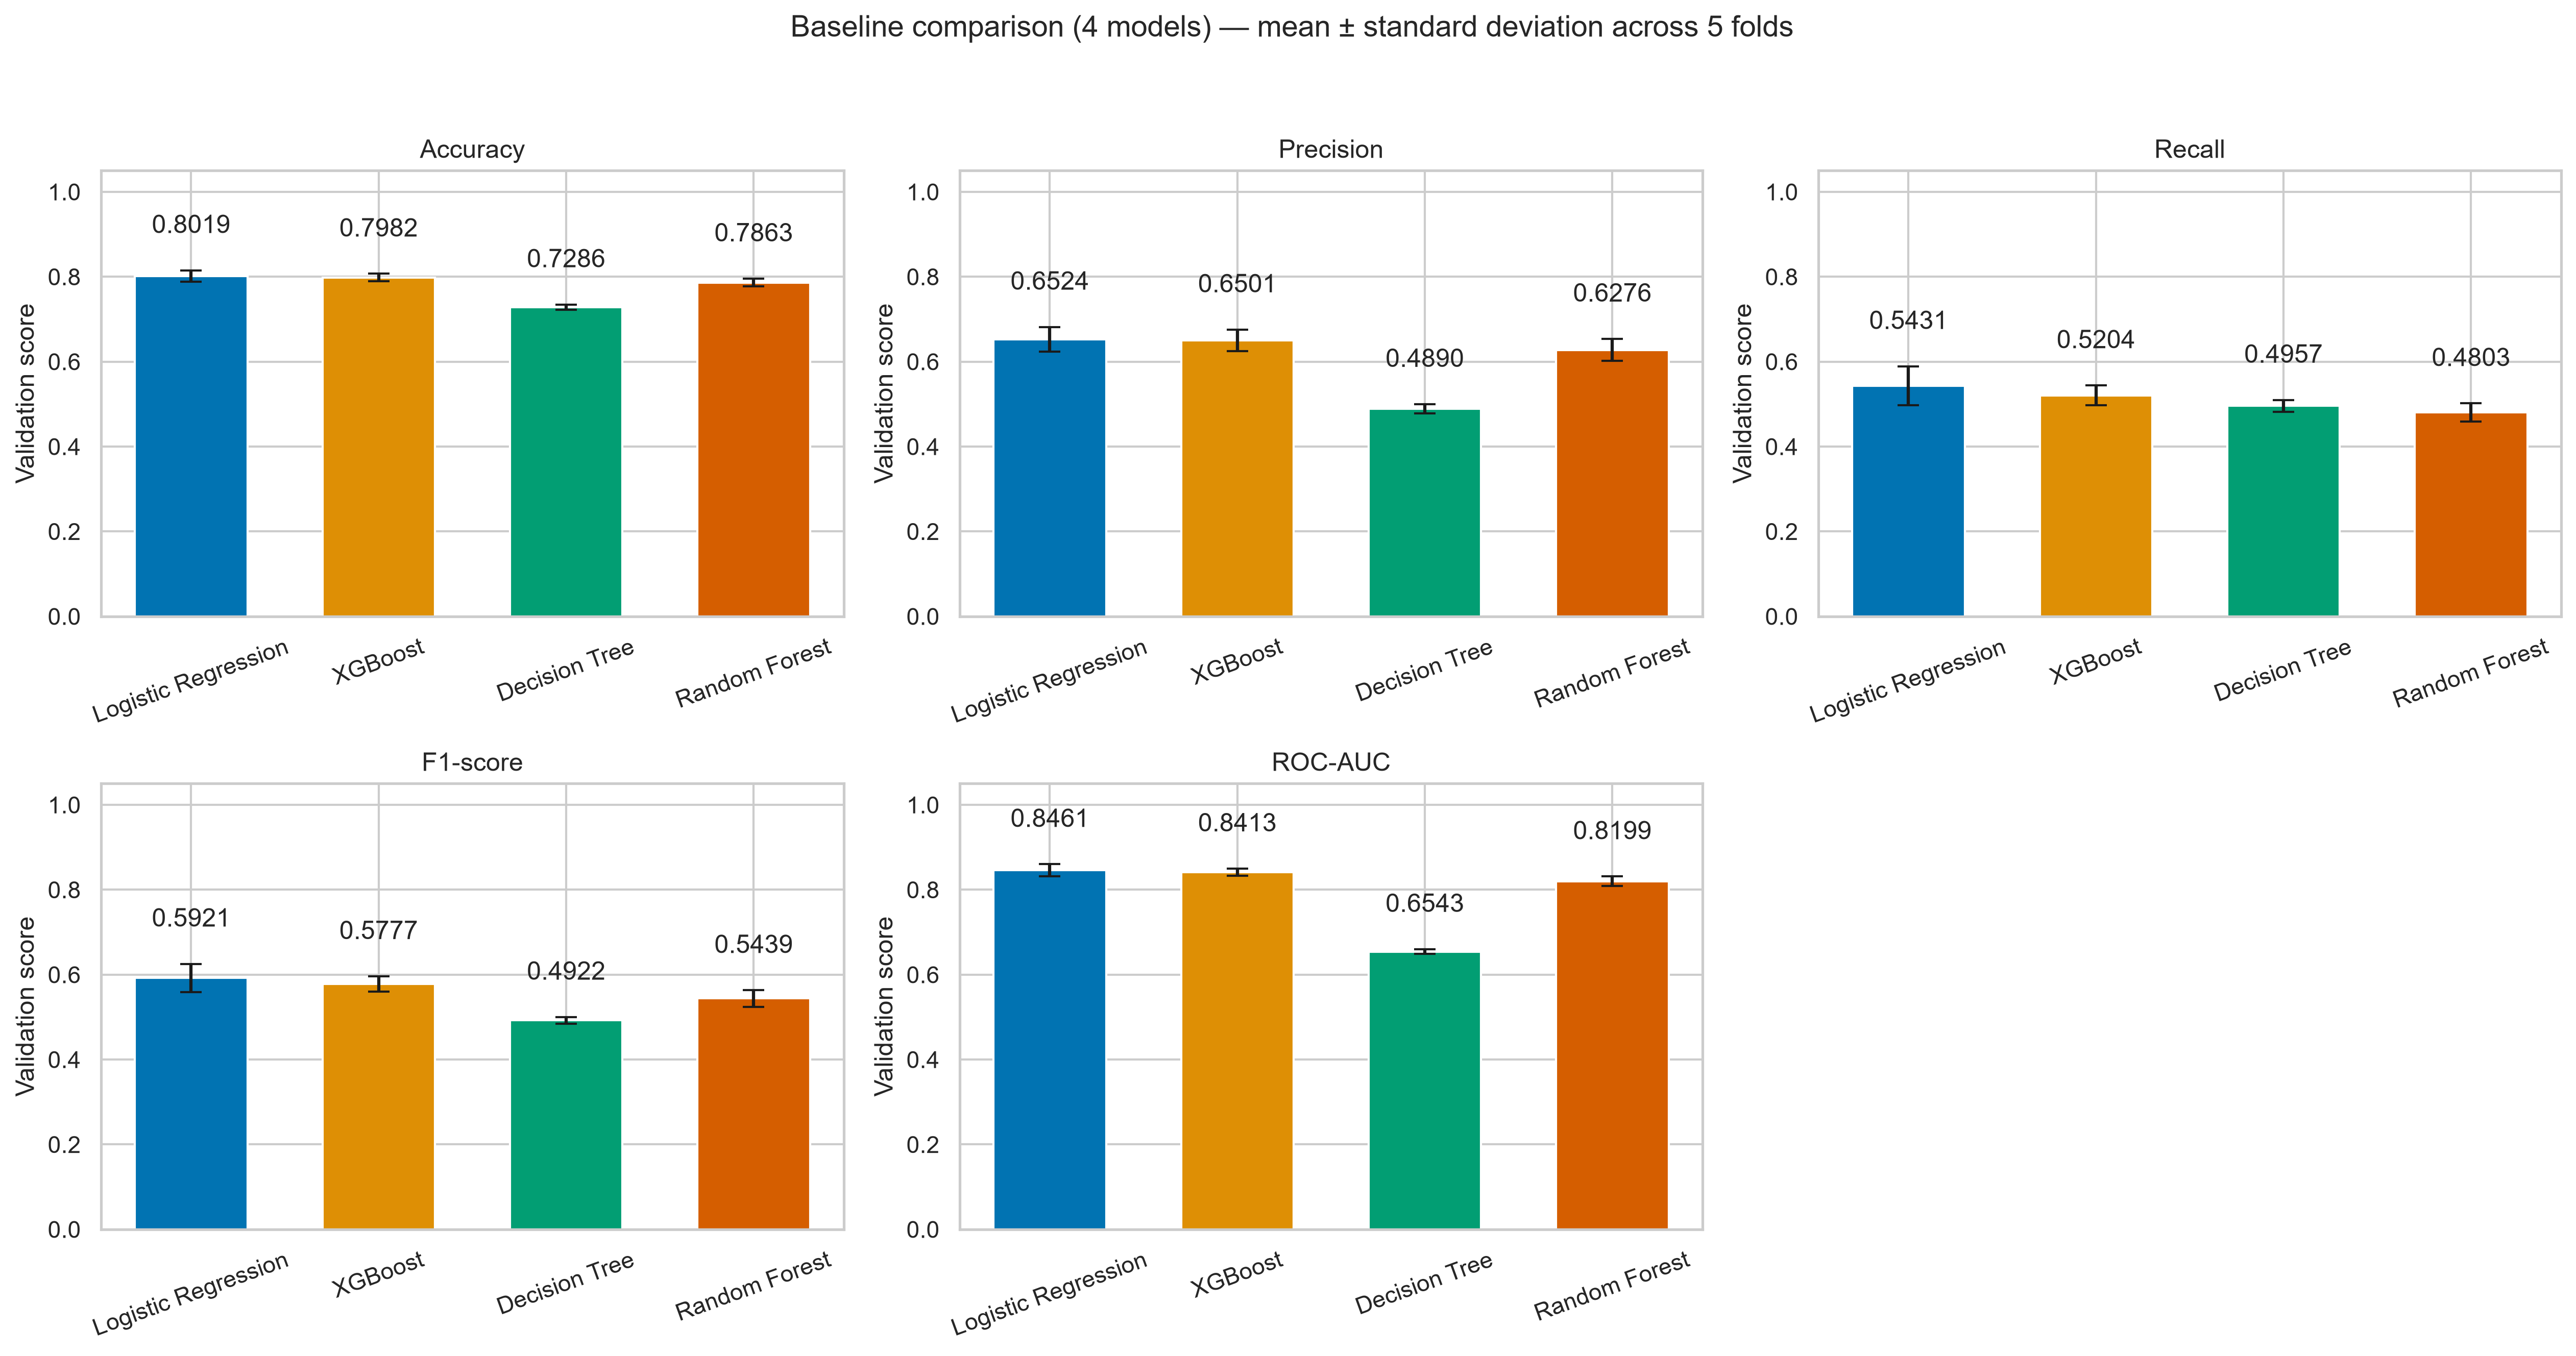
\includegraphics[width=\textwidth]{img/baseline_validation_all_models.png}
\caption{So sánh các chỉ số validation của 4 mô hình baseline (thanh lỗi: độ lệch chuẩn qua 5 fold)}
\end{figure}

Nhận xét:
\begin{itemize}
    \item Theo F1 và ROC-AUC, thứ tự các mô hình là: \textbf{Logistic Regression $>$ XGBoost $>$ Random Forest $>$ Decision Tree}. Ở cấu hình mặc định, các mô hình dựa trên cây chưa vượt được mô hình tuyến tính.
    \item Logistic Regression và XGBoost rất gần nhau (chênh lệch F1 khoảng 0,014 và ROC-AUC khoảng 0,005, nhỏ hơn độ lệch chuẩn giữa các fold), nên chưa thể kết luận mô hình nào tốt hơn.
    \item Random Forest thấp hơn Logistic Regression khoảng 0,05 ở F1 và 0,026 ở ROC-AUC. Decision Tree thấp hơn hẳn, đặc biệt ROC-AUC chỉ 0,654 do cây không giới hạn độ sâu cho xác suất gần như chỉ nhận giá trị 0 hoặc 1.
    \item \textbf{Recall của cả bốn mô hình chỉ khoảng 0,48--0,54}: với ngưỡng mặc định 0,5, mô hình mới phát hiện được khoảng một nửa số khách hàng thực sự rời bỏ. Đây là điểm yếu chung cần cải thiện ở các thực nghiệm sau.
\end{itemize}

\subsubsection{Phân tích overfitting}

\begin{table}[H]
\centering
\begin{tabular}{lcccccc}
\toprule
\textbf{Mô hình} & \textbf{F1 train} & \textbf{F1 val} & \textbf{F1 gap} & \textbf{AUC train} & \textbf{AUC val} & \textbf{AUC gap} \\
\midrule
Logistic Regression & 0,6018 & 0,5921 & 0,0096 & 0,8496 & 0,8461 & 0,0035 \\
XGBoost             & 0,7602 & 0,5777 & 0,1825 & 0,9504 & 0,8413 & 0,1091 \\
Random Forest       & 0,9968 & 0,5439 & 0,4529 & 0,9999 & 0,8199 & 0,1801 \\
Decision Tree       & 0,9968 & 0,4922 & 0,5046 & 1,0000 & 0,6543 & 0,3457 \\
\bottomrule
\end{tabular}
\caption{Khoảng cách giữa điểm train và validation (trung bình 5 fold)}
\end{table}

\begin{figure}[H]
\centering
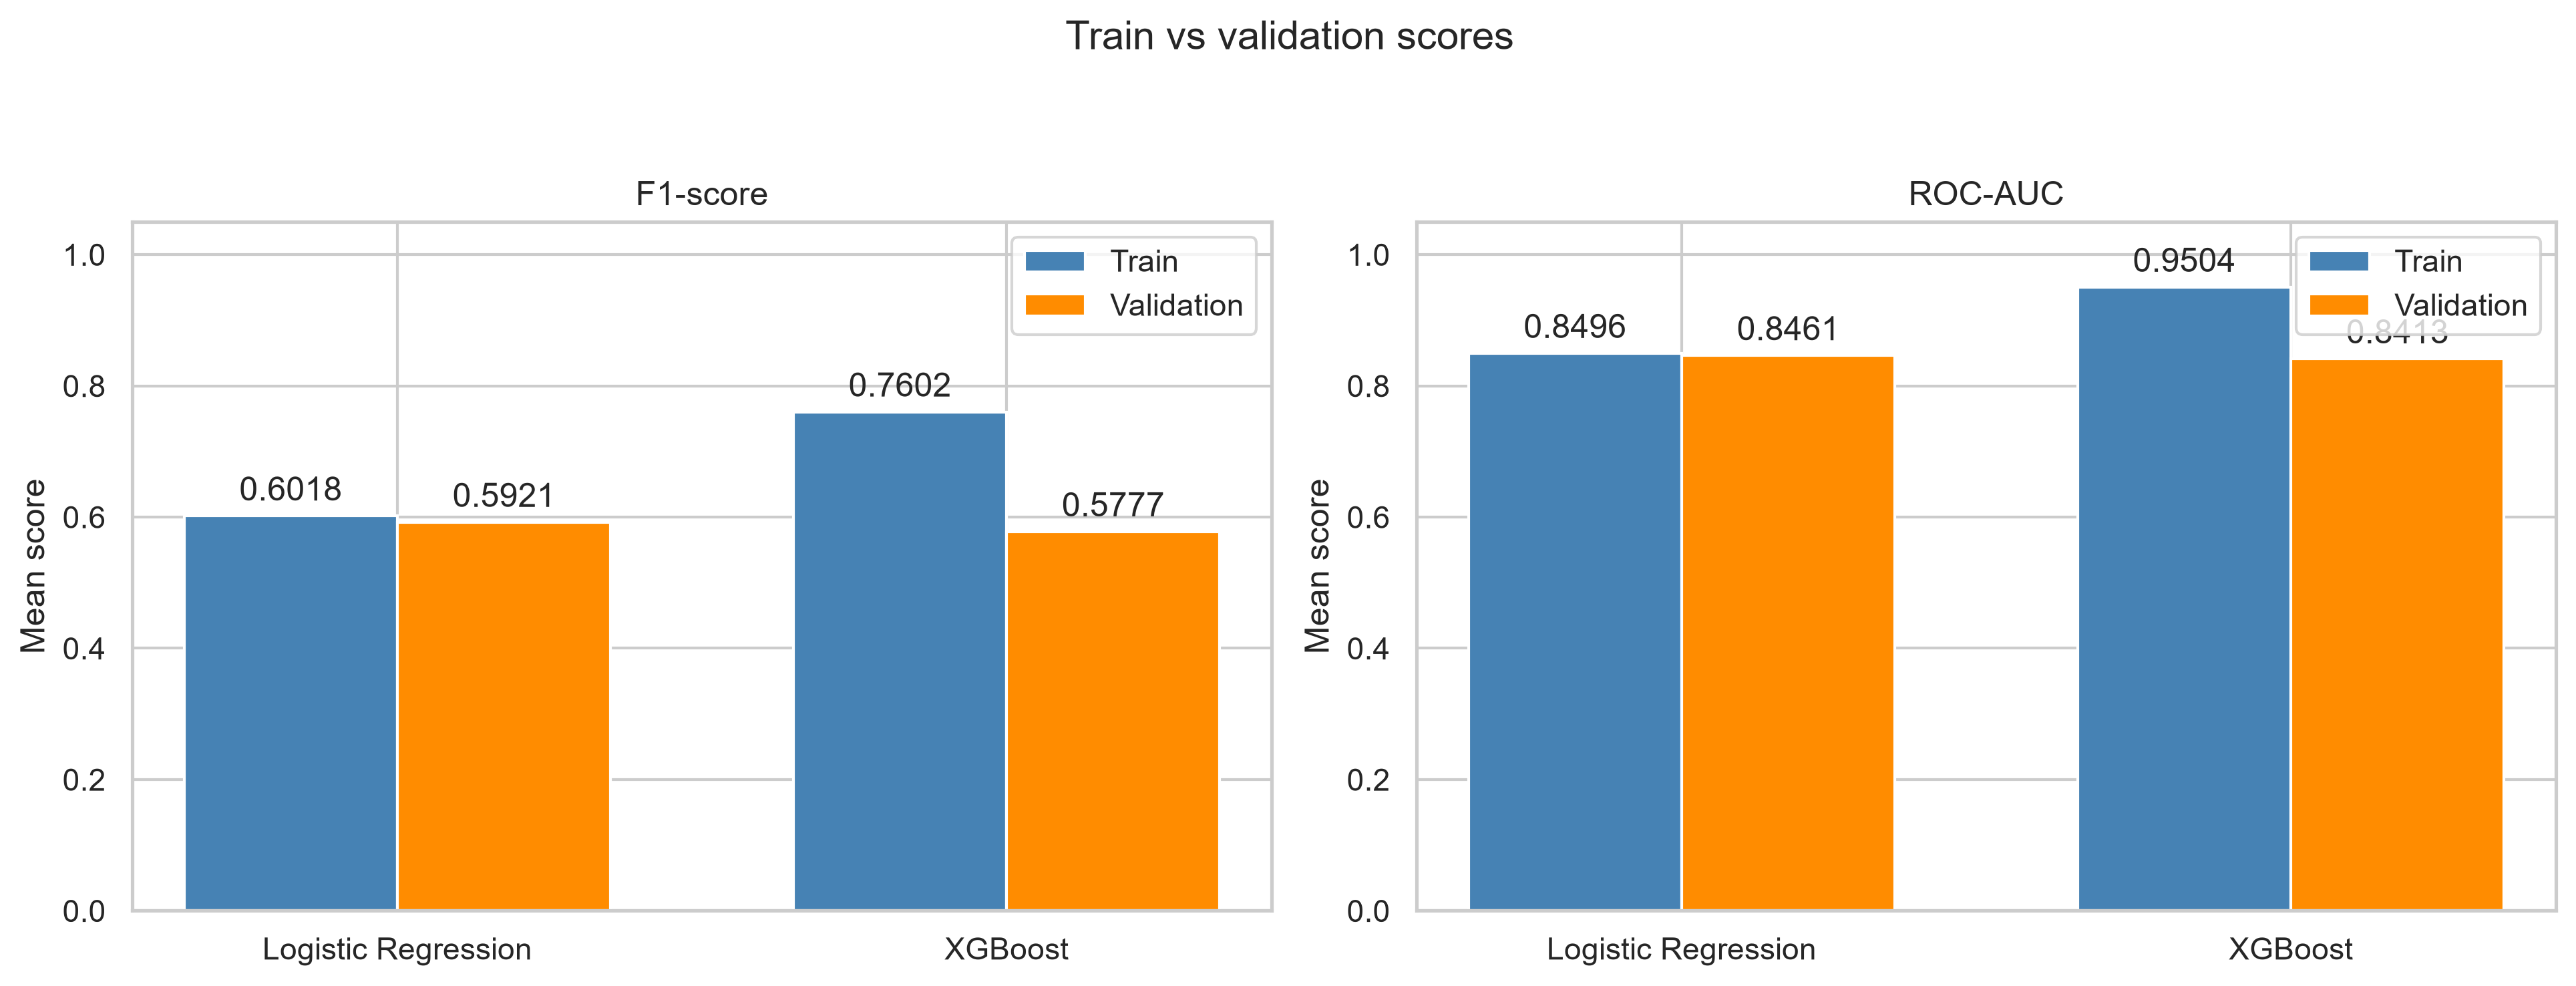
\includegraphics[width=0.49\textwidth]{img/train_vs_val_lr_xgb.png}
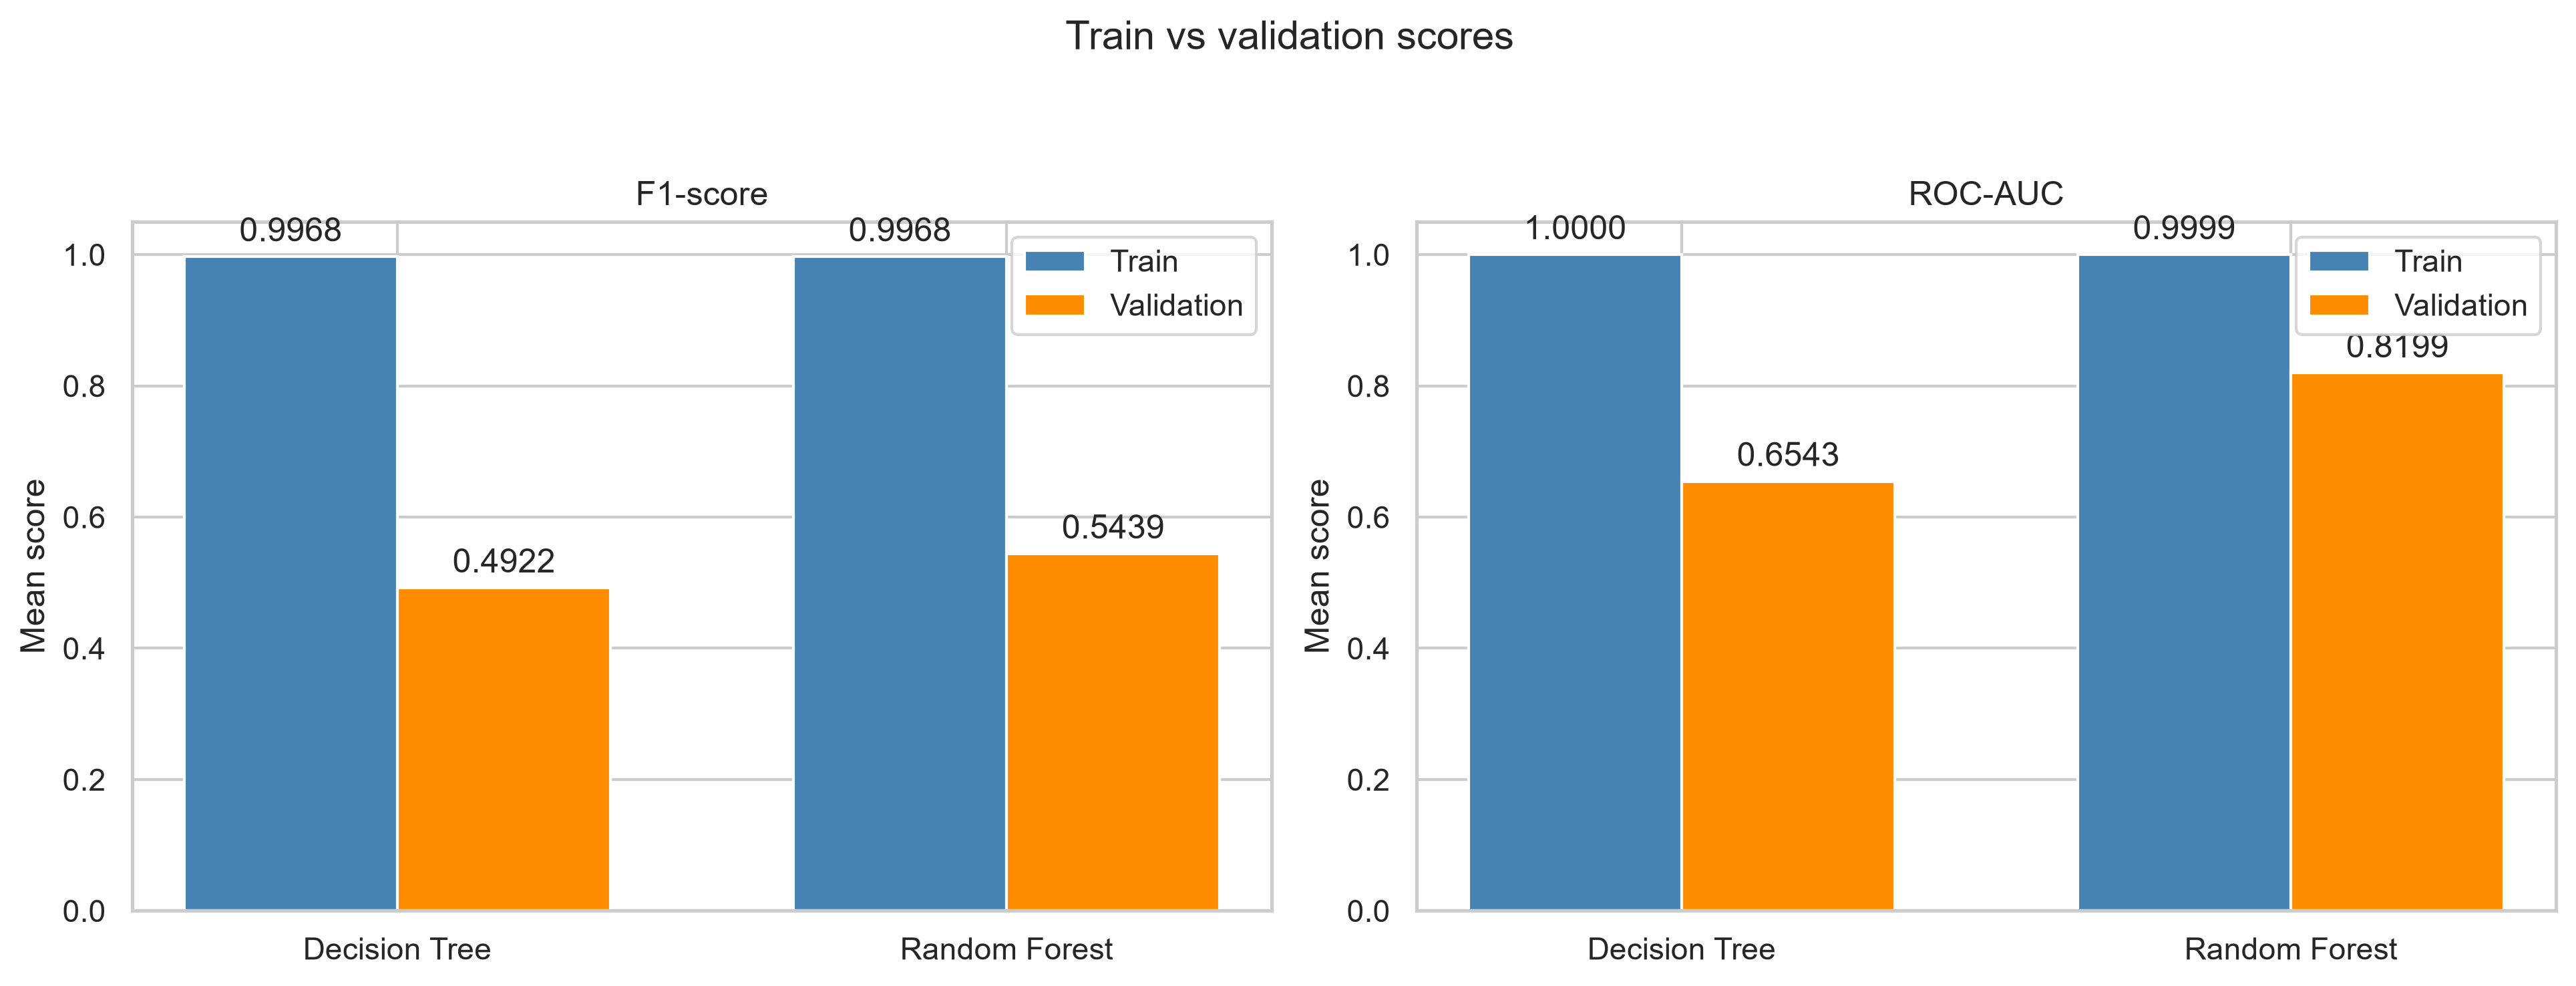
\includegraphics[width=0.49\textwidth]{img/train_vs_val_dt_rf.png}
\caption{F1 và ROC-AUC trên train và validation: Logistic Regression, XGBoost (trái); Decision Tree, Random Forest (phải)}
\end{figure}

\begin{itemize}
    \item \textbf{Logistic Regression} có điểm train và validation gần như trùng nhau: mô hình không overfit, nhưng điểm train thấp cho thấy mô hình tuyến tính có thể đang bị giới hạn về khả năng biểu diễn (\textit{underfit} nhẹ).
    \item \textbf{Decision Tree} và \textbf{Random Forest} gần như ghi nhớ hoàn toàn tập huấn luyện (F1 train $\approx 0{,}997$) do cây phát triển không giới hạn đến khi mỗi lá gần như thuần nhất. Random Forest giảm phương sai nhờ lấy trung bình nhiều cây (ROC-AUC validation tăng từ 0,654 lên 0,820) nhưng từng cây thành phần vẫn overfit.
    \item \textbf{XGBoost} cũng có dấu hiệu overfitting (F1 gap 0,18) ở cấu hình \texttt{max\_depth=6}, 100 cây.
    \item Kết luận: các mô hình cây có nhiều dư địa cải thiện nhất thông qua việc \textbf{giới hạn độ phức tạp} (\texttt{max\_depth}, \texttt{min\_samples\_leaf}, \texttt{min\_samples\_split}) và chính quy hóa -- là trọng tâm của Experiment 4.
\end{itemize}

\subsubsection{Độ ổn định qua các fold}

\begin{figure}[H]
\centering
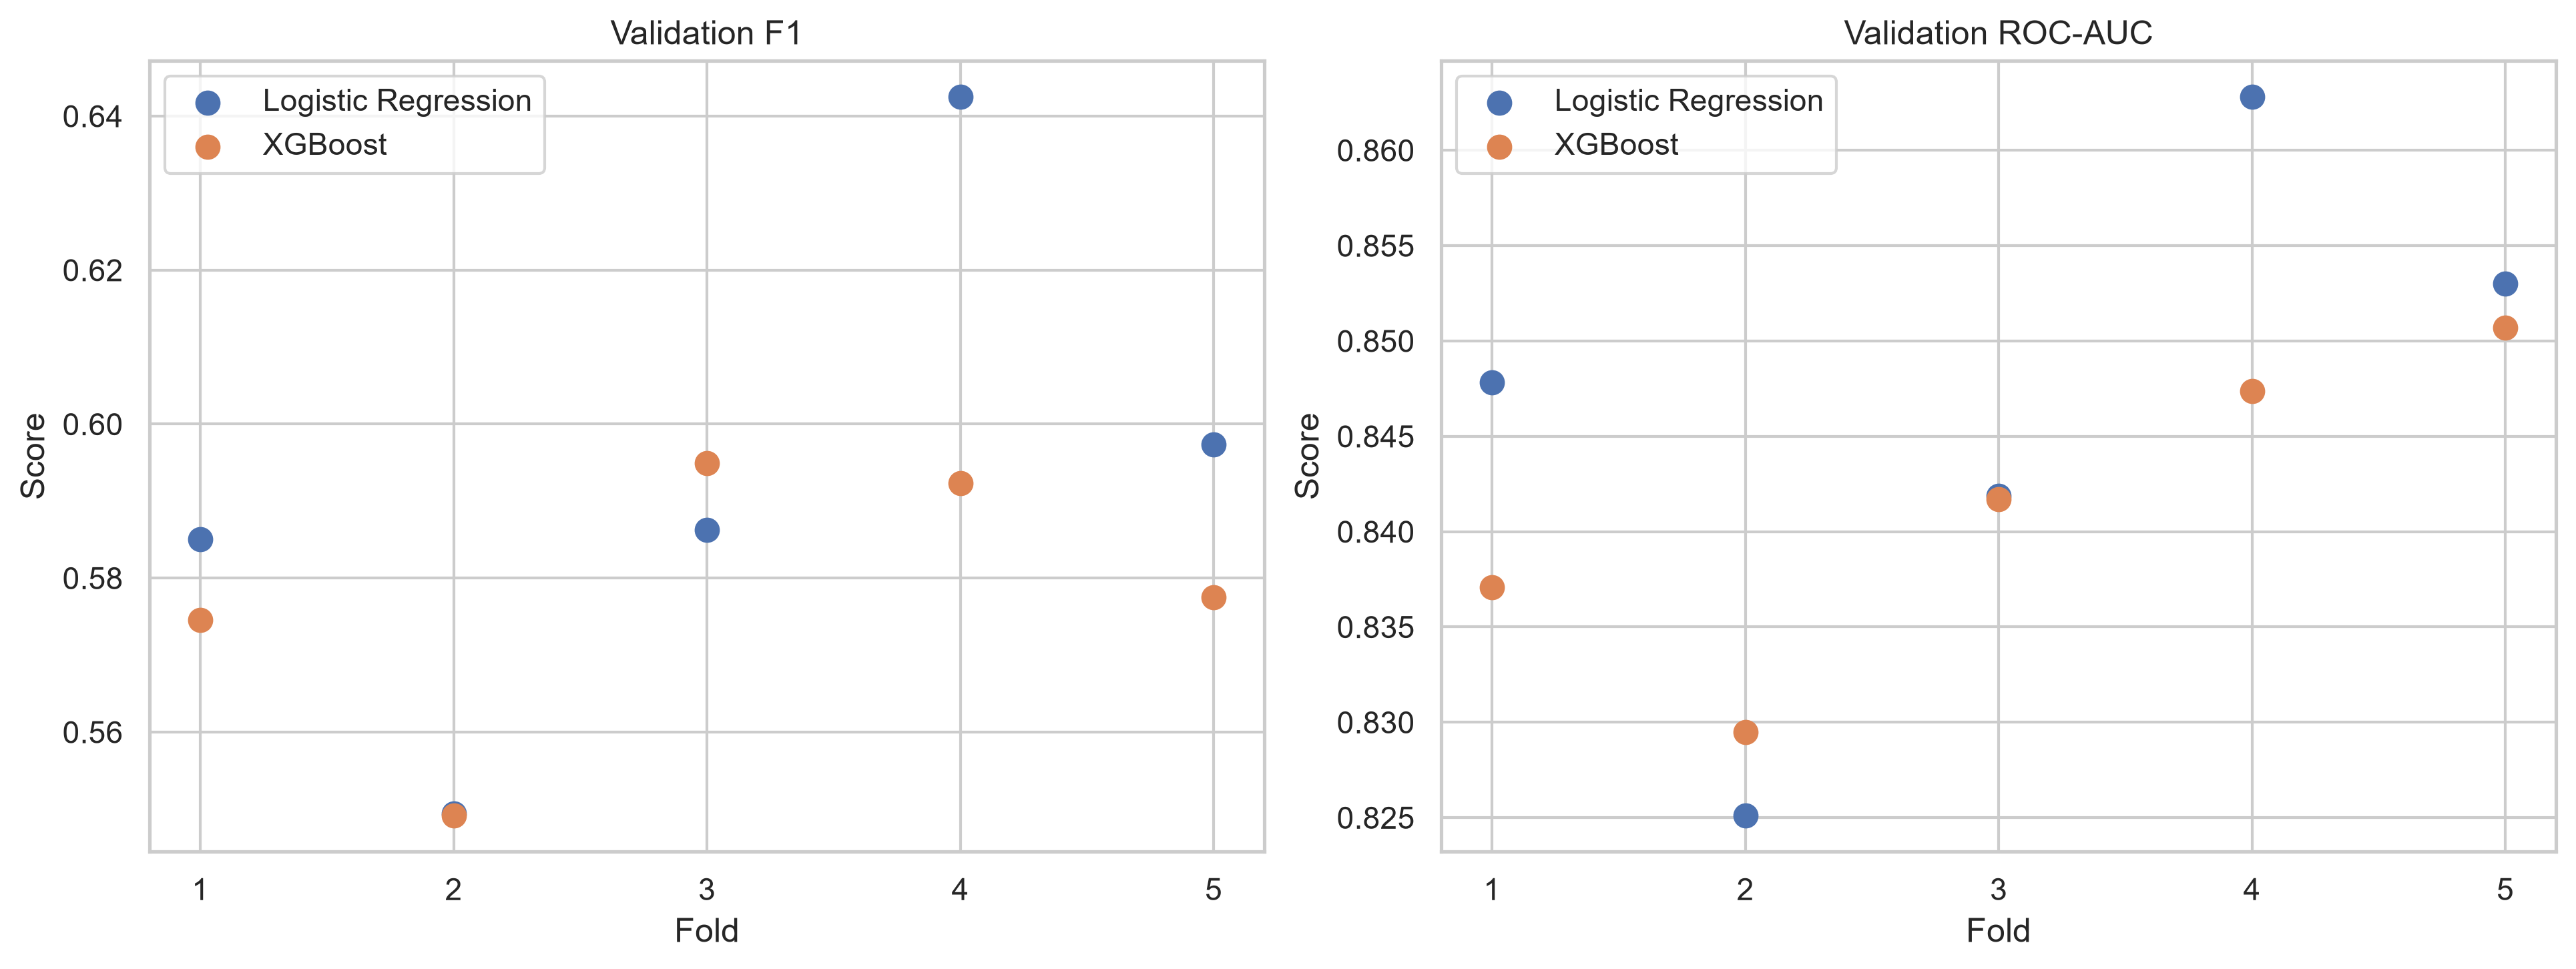
\includegraphics[width=0.49\textwidth]{img/folds_lr_xgb.png}
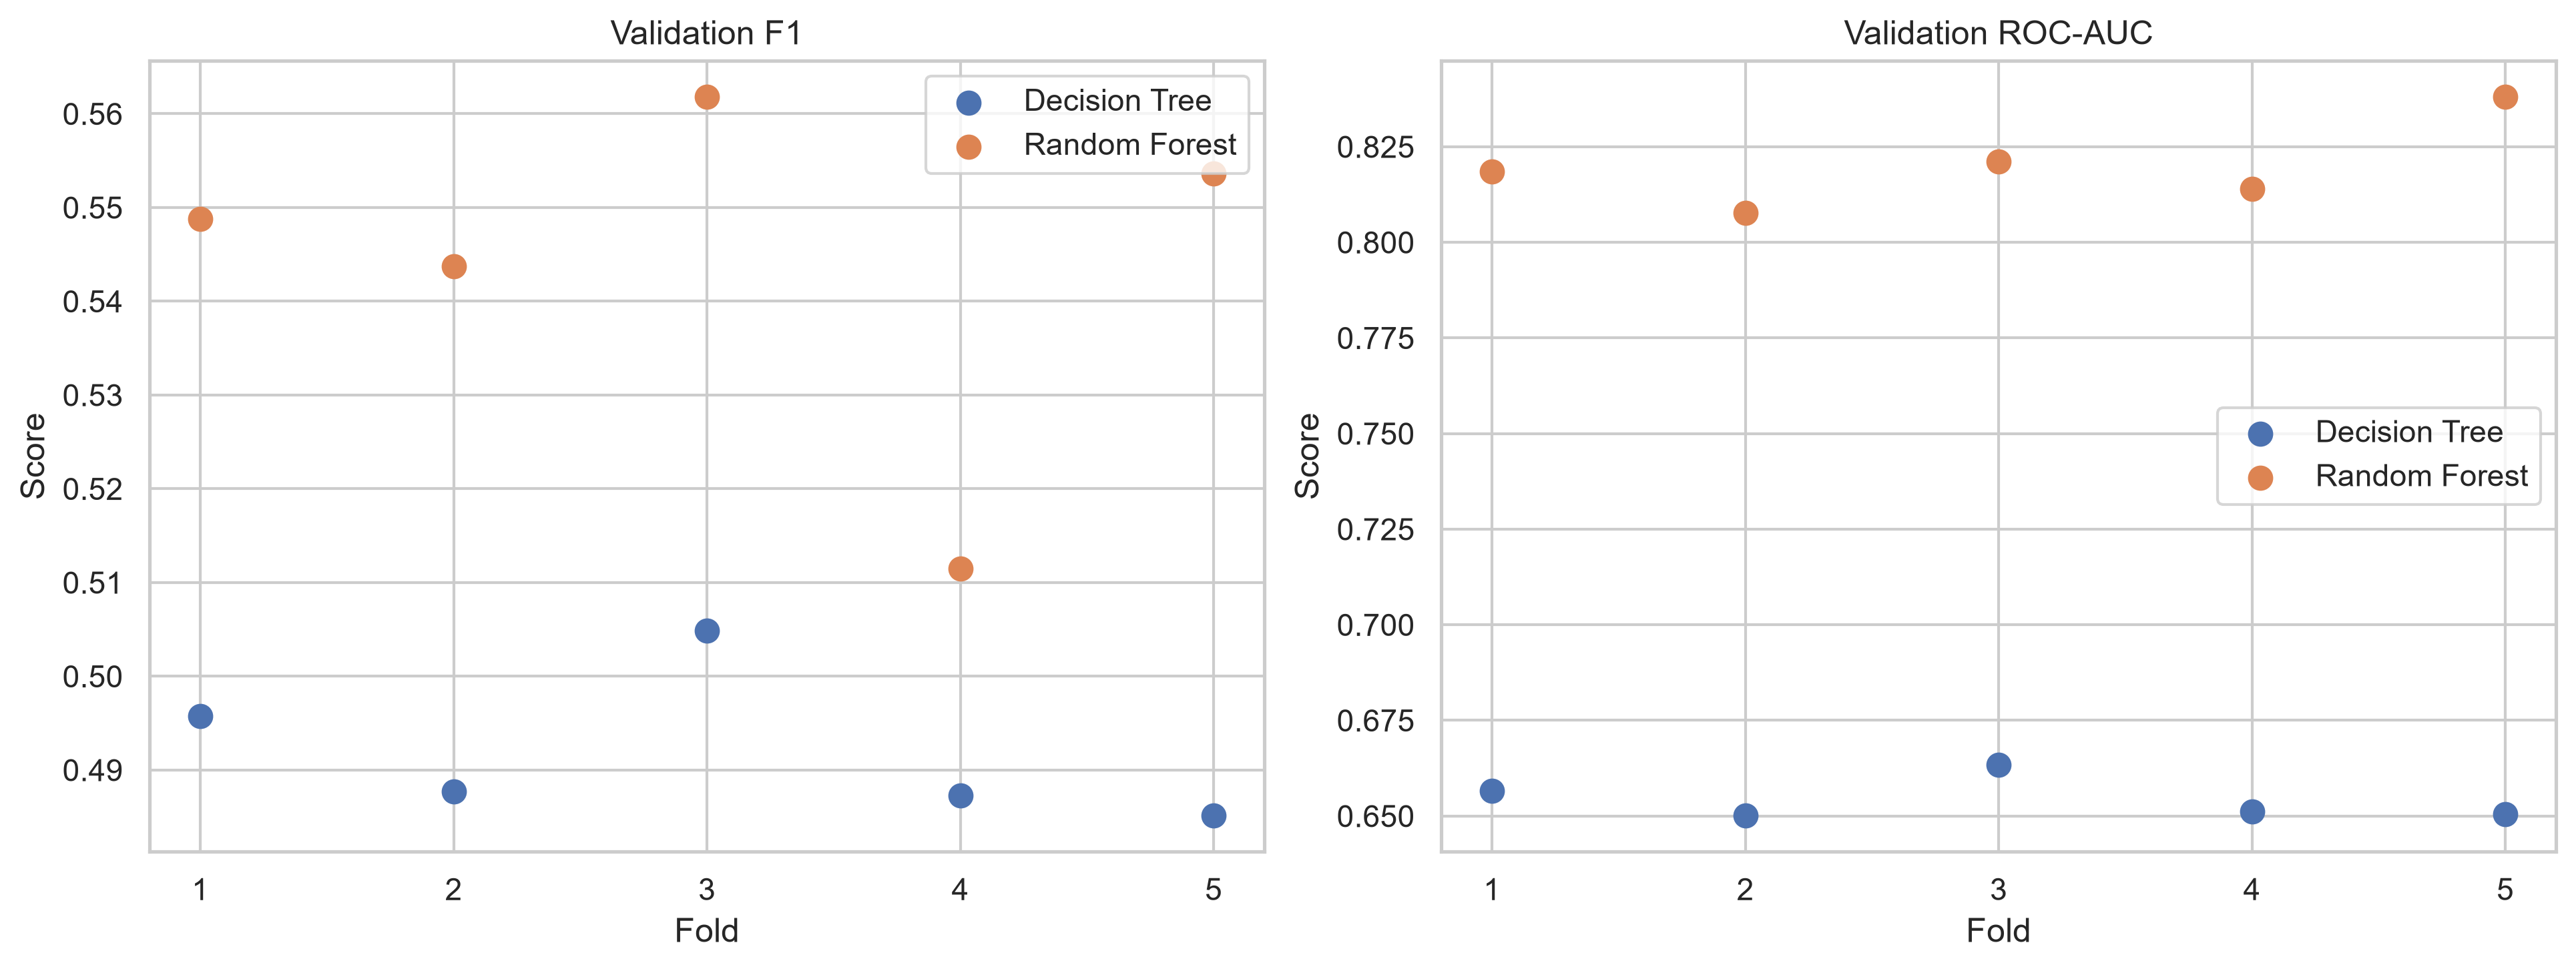
\includegraphics[width=0.49\textwidth]{img/folds_dt_rf.png}
\caption{F1 và ROC-AUC validation trên từng fold}
\end{figure}

Thứ hạng các mô hình tương đối nhất quán qua các fold: Random Forest luôn có ROC-AUC cao hơn Decision Tree ở cả 5 fold (0,808--0,838 so với 0,650--0,663). Logistic Regression có mức dao động F1 lớn nhất (0,550--0,643), trong khi XGBoost ổn định hơn nhưng có điểm trung bình thấp hơn một chút.

\subsubsection{PR-AUC của các mô hình baseline}
Với dữ liệu mất cân bằng, nhóm ghi thêm PR-AUC cho mọi lần chạy. Ở cấu hình baseline, PR-AUC của Logistic Regression là 0,662, XGBoost 0,653, Random Forest 0,610 và Decision Tree chỉ 0,377 (mức ngẫu nhiên khoảng 0,265). Thứ hạng giống với F1 và ROC-AUC.

% ============================================================
\subsection{Experiment 2: Ảnh hưởng của Feature Engineering}
% ============================================================
\textbf{Thiết kế:} thêm bước \texttt{ChurnFeatureEngineer} (9 đặc trưng mới, Mục 3) vào đầu pipeline, giữ nguyên mọi thứ khác (\texttt{python -m src.train cv --feature-engineering}). Để kiểm tra FE có giúp ích khi đã xử lý mất cân bằng hay không, nhóm chạy FE trong cả ba bối cảnh: không xử lý, class weight và SMOTE. Mỗi so sánh được thực hiện \textbf{theo cặp trên từng fold} (\texttt{src/compare.py}): vì mọi lần chạy dùng cùng 5 fold, chênh lệch được tính trên từng fold rồi lấy trung bình, kèm số fold mà cấu hình có FE tốt hơn.

\begin{table}[H]
\centering
\small
\begin{tabular}{lcccccc}
\toprule
\multirow{2}{*}{\textbf{Mô hình}} & \multicolumn{2}{c}{\textbf{Không xử lý}} & \multicolumn{2}{c}{\textbf{Class weight}} & \multicolumn{2}{c}{\textbf{SMOTE}} \\
\cmidrule(lr){2-3} \cmidrule(lr){4-5} \cmidrule(lr){6-7}
 & $\Delta$F1 & $\Delta$PR-AUC & $\Delta$F1 & $\Delta$PR-AUC & $\Delta$F1 & $\Delta$PR-AUC \\
\midrule
Logistic Regression & +0,003 (3/5) & +0,001 (3/5) & +0,001 (2/5) & +0,001 (3/5) & +0,000 (2/5) & $-$0,000 (2/5) \\
Decision Tree & +0,003 (3/5) & +0,003 (3/5) & $-$0,009 (1/5) & $-$0,008 (2/5) & +0,005 (3/5) & +0,003 (3/5) \\
Random Forest & $-$0,010 (2/5) & +0,008 (3/5) & $-$0,005 (1/5) & +0,007 (4/5) & +0,010 (3/5) & +0,007 (4/5) \\
XGBoost & $-$0,012 (1/5) & $-$0,007 (1/5) & $-$0,004 (3/5) & $-$0,003 (3/5) & $-$0,010 (1/5) & $-$0,006 (1/5) \\
\bottomrule
\end{tabular}
\caption{Chênh lệch khi thêm Feature Engineering (trung bình 5 fold; trong ngoặc: số fold cải thiện)}
\label{tab:fe}
\end{table}

\subsubsection{Phân tích}
\begin{itemize}
    \item \textbf{Feature Engineering không mang lại cải thiện đáng kể.} Mọi chênh lệch đều nằm trong khoảng $\pm 0{,}012$, nhỏ hơn độ lệch chuẩn của F1 giữa các fold (0,02--0,03), và không có cấu hình nào cải thiện ở cả 5 fold. Kết quả nhất quán trong cả ba bối cảnh xử lý mất cân bằng.
    \item \textbf{XGBoost giảm nhẹ trong cả ba bối cảnh} (F1 giảm 0,004--0,012, chỉ cải thiện ở 1--3/5 fold). Ở cấu hình mặc định (\texttt{max\_depth=6}), XGBoost đã overfit (Mục 5.1); thêm các đặc trưng liên tục như \texttt{avg\_monthly\_charge}, \texttt{charge\_diff} tạo thêm điểm chia để mô hình khớp nhiễu. F1 train của XGBoost tăng từ 0,760 lên 0,790 trong khi F1 validation giảm.
    \item \textbf{Random Forest tăng nhẹ PR-AUC} (+0,007 đến +0,008, cải thiện ở 3--4/5 fold) nhưng F1 lúc tăng lúc giảm, nên không đủ cơ sở kết luận.
    \item \textbf{Nguyên nhân:} các đặc trưng mới đều được dựng từ thông tin mô hình đã có. Mô hình cây tự học được các ngưỡng (ví dụ \texttt{tenure} $\le 12$) và tương tác (hợp đồng $\times$ thời gian sử dụng), còn Logistic Regression đã nắm được xu hướng chính qua \texttt{tenure}, \texttt{Contract} và \texttt{InternetService}.
    \item \textbf{Kết luận:} FE không được đưa vào cấu hình cuối cùng; các thực nghiệm sau dùng 19 đặc trưng gốc.
\end{itemize}

% ============================================================
\subsection{Experiment 3: Xử lý mất cân bằng dữ liệu}
% ============================================================
\textbf{Thiết kế:} giữ nguyên 19 đặc trưng gốc và siêu tham số baseline, chỉ thay đổi cách xử lý mất cân bằng (\texttt{--imbalance}):
\begin{itemize}
    \item \textbf{Class weight:} \texttt{class\_weight="balanced"} cho Logistic Regression, Decision Tree, Random Forest; với XGBoost dùng \texttt{scale\_pos\_weight} bằng tỉ lệ số mẫu không rời bỏ / rời bỏ ($4.139 / 1.495 \approx 2{,}77$). Cả hai cách đều làm tổng trọng số của hai lớp bằng nhau.
    \item \textbf{SMOTE:} chèn bước \texttt{SMOTE} sau \texttt{preprocessor} trong \texttt{imblearn.pipeline.Pipeline}. Pipeline của \texttt{imblearn} chỉ sinh mẫu khi \texttt{fit}, nên SMOTE chỉ tác động lên phần huấn luyện của mỗi fold; fold validation và tập test giữ nguyên phân bố thật.
\end{itemize}

\begin{table}[H]
\centering
\small
\begin{tabular}{llccccc}
\toprule
\textbf{Mô hình} & \textbf{Chiến lược} & \textbf{Precision} & \textbf{Recall} & \textbf{F1} & \textbf{$\Delta$F1 (fold)} & \textbf{PR-AUC} \\
\midrule
\multirow{3}{*}{Logistic Regression} & Không xử lý & 0,652 & 0,543 & 0,592 & -- & 0,662 \\
 & Class weight & 0,517 & \textbf{0,801} & 0,628 & +0,036 (5/5) & 0,660 \\
 & SMOTE & 0,526 & 0,789 & \textbf{0,631} & +0,039 (5/5) & 0,658 \\
\midrule
\multirow{3}{*}{Decision Tree} & Không xử lý & 0,489 & 0,496 & 0,492 & -- & 0,377 \\
 & Class weight & 0,512 & 0,496 & \textbf{0,504} & +0,012 (4/5) & 0,389 \\
 & SMOTE & 0,479 & 0,495 & 0,487 & $-$0,006 (1/5) & 0,372 \\
\midrule
\multirow{3}{*}{Random Forest} & Không xử lý & 0,628 & 0,480 & 0,544 & -- & 0,610 \\
 & Class weight & 0,563 & \textbf{0,638} & \textbf{0,598} & +0,054 (5/5) & 0,604 \\
 & SMOTE & 0,608 & 0,496 & 0,546 & +0,002 (3/5) & 0,593 \\
\midrule
\multirow{3}{*}{XGBoost} & Không xử lý & 0,650 & 0,520 & 0,578 & -- & 0,653 \\
 & Class weight & 0,545 & \textbf{0,747} & \textbf{0,630} & +0,053 (5/5) & 0,653 \\
 & SMOTE & 0,636 & 0,565 & 0,598 & +0,020 (5/5) & 0,651 \\
\bottomrule
\end{tabular}
\caption{Kết quả validation (5-fold CV, ngưỡng 0,5) của các chiến lược xử lý mất cân bằng}
\label{tab:imbalance}
\end{table}

\subsubsection{Phân tích}
\begin{itemize}
    \item \textbf{Class weight là chiến lược tốt và ổn định nhất.} F1 tăng 0,036--0,054 và tăng ở cả 5/5 fold với Logistic Regression, Random Forest và XGBoost. Recall tăng mạnh: Logistic Regression từ 0,543 lên 0,801, XGBoost từ 0,520 lên 0,747. Mô hình giờ phát hiện được khoảng 3/4 khách hàng rời bỏ thay vì một nửa.
    \item \textbf{Cái giá là Precision giảm} (Logistic Regression: 0,652 xuống 0,517; XGBoost: 0,650 xuống 0,545): mô hình chấp nhận cảnh báo nhầm nhiều hơn để bắt được nhiều khách hàng rời bỏ hơn. Vì Recall tăng nhiều hơn Precision giảm, F1 vẫn tăng. Với bài toán giữ chân khách hàng, bỏ sót một khách hàng sắp rời bỏ thường tốn kém hơn gửi nhầm một ưu đãi, nên đánh đổi này là hợp lý.
    \item \textbf{PR-AUC gần như không đổi} ($|\Delta| \le 0{,}006$ với LR, RF, XGBoost). Class weight không làm mô hình \textit{xếp hạng} khách hàng tốt hơn mà chủ yếu \textit{dịch chuyển xác suất dự đoán} lên cao, tương đương với hạ ngưỡng quyết định.
    \item \textbf{SMOTE hiệu quả với Logistic Regression} (+0,039 F1, tương đương class weight) nhưng yếu hơn với mô hình cây: XGBoost chỉ +0,020, Random Forest gần như không đổi. SMOTE nội suy tuyến tính giữa các mẫu sau One-Hot Encoding nên tạo ra các giá trị không có thật (ví dụ 0,4 cho cột \texttt{Contract\_Two year}); mô hình cây chia theo ngưỡng nên dễ bị ảnh hưởng bởi các mẫu giả này. Class weight đơn giản hơn và không sinh dữ liệu giả.
    \item \textbf{Decision Tree gần như không phản ứng} (Recall vẫn 0,496), và Recall của Random Forest chỉ tăng lên 0,638. Ở cấu hình mặc định, cây phát triển đến khi lá thuần nhất (F1 train $\approx 0{,}997$), nên xác suất dự đoán gần như chỉ là 0 hoặc 1; trọng số lớp không còn tác dụng khi mọi lá đã thuần nhất. Điều này chỉ thay đổi sau khi giới hạn độ phức tạp ở Experiment 4.
    \item \textbf{Kết luận:} chọn \textbf{class weight} cho mọi mô hình ở các bước tiếp theo.
\end{itemize}

% ============================================================
\subsection{Experiment 4: Hyperparameter Tuning}
% ============================================================
\textbf{Thiết kế:} tối ưu siêu tham số bằng \texttt{RandomizedSearchCV} (\texttt{python -m src.tune}) trên cấu hình class weight, 19 đặc trưng gốc. Tìm kiếm dùng đúng 5 fold của các thực nghiệm trước, nên kết quả so sánh cặp được với Experiment 3. Tiêu chí chọn là \textbf{PR-AUC} vì chỉ số này không phụ thuộc ngưỡng và tập trung vào lớp rời bỏ; ngưỡng được chọn riêng ở Experiment 5.

\begin{table}[H]
\centering
\small
\begin{tabular}{l c p{9.8cm}}
\toprule
\textbf{Mô hình} & \textbf{Số tổ hợp} & \textbf{Không gian tìm kiếm} \\
\midrule
Logistic Regression & 30 & \texttt{C} $\sim$ log-uniform$(10^{-3}, 10^{2})$ \\
Decision Tree & 50 & \texttt{max\_depth} $\in [2, 15]$, \texttt{min\_samples\_leaf} $\in [1, 59]$, \texttt{criterion} $\in$ \{gini, entropy\} \\
Random Forest & 40 & \texttt{n\_estimators} $\in [200, 600]$, \texttt{max\_depth} $\in$ \{4, 6, 8, 10, 12, 16, None\}, \texttt{min\_samples\_leaf} $\in [1, 29]$, \texttt{max\_features} $\in$ \{sqrt, log2, 0,5\} \\
XGBoost & 60 & \texttt{n\_estimators} $\in [100, 600]$, \texttt{learning\_rate} $\sim$ log-uniform$(0{,}01; 0{,}3)$, \texttt{max\_depth} $\in [2, 7]$, \texttt{min\_child\_weight} $\in [1, 10]$, \texttt{subsample}, \texttt{colsample\_bytree} $\in [0{,}6; 1]$, \texttt{reg\_lambda} $\sim$ log-uniform$(0{,}1; 10)$ \\
\bottomrule
\end{tabular}
\caption{Không gian tìm kiếm siêu tham số}
\end{table}

\begin{table}[H]
\centering
\small
\begin{tabular}{l p{10cm}}
\toprule
\textbf{Mô hình} & \textbf{Siêu tham số tốt nhất} \\
\midrule
Logistic Regression & \texttt{C=0,92} \\
Decision Tree & \texttt{criterion=entropy}, \texttt{max\_depth=12}, \texttt{min\_samples\_leaf=51} \\
Random Forest & 287 cây, \texttt{max\_depth=8}, \texttt{max\_features=0,5}, \texttt{min\_samples\_leaf=11} \\
XGBoost & 271 cây, \texttt{max\_depth=3}, \texttt{learning\_rate=0,023}, \texttt{min\_child\_weight=5}, \texttt{subsample=0,82}, \texttt{colsample\_bytree=0,96}, \texttt{reg\_lambda=0,79} \\
\bottomrule
\end{tabular}
\caption{Siêu tham số tốt nhất theo PR-AUC}
\end{table}

\subsubsection{Kết quả}

\begin{table}[H]
\centering
\small
\begin{tabular}{lcccccc}
\toprule
\textbf{Mô hình} & \textbf{Recall} & \textbf{F1} & \textbf{$\Delta$F1 (fold)} & \textbf{ROC-AUC} & \textbf{PR-AUC} & \textbf{$\Delta$PR-AUC (fold)} \\
\midrule
Logistic Regression & 0,801 & 0,628 & +0,000 (2/5) & 0,846 & 0,660 & +0,000 (5/5) \\
Decision Tree & 0,799 & 0,621 & \textbf{+0,117 (5/5)} & 0,830 & 0,630 & \textbf{+0,242 (5/5)} \\
Random Forest & 0,776 & 0,631 & +0,033 (5/5) & 0,848 & 0,667 & +0,063 (5/5) \\
XGBoost & \textbf{0,806} & \textbf{0,632} & +0,002 (3/5) & \textbf{0,850} & \textbf{0,671} & +0,018 (5/5) \\
\bottomrule
\end{tabular}
\caption{Kết quả validation sau tuning (class weight, ngưỡng 0,5). Chênh lệch so với class weight với siêu tham số mặc định (Experiment 3).}
\label{tab:tuning}
\end{table}

\begin{figure}[H]
\centering
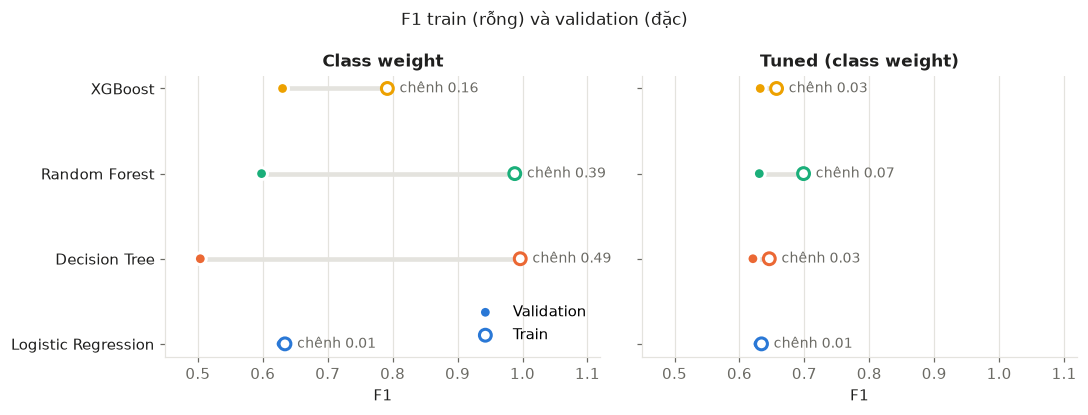
\includegraphics[width=\textwidth]{img/nb_train_val_gap.png}
\caption{F1 trên phần huấn luyện (vòng rỗng) và validation (chấm đặc) của mỗi fold, trước (trái) và sau tuning (phải)}
\label{fig:tuning_gap}
\end{figure}

\subsubsection{Phân tích}
\begin{itemize}
    \item \textbf{Tuning giải quyết được overfitting của mô hình cây.} Khoảng cách F1 train--validation giảm từ 0,49 xuống 0,03 với Decision Tree, từ 0,39 xuống 0,07 với Random Forest và từ 0,16 xuống 0,03 với XGBoost (Hình~\ref{fig:tuning_gap}). Các cấu hình được chọn đều đơn giản hơn mặc định: lá có ít nhất 11--51 mẫu, cây sâu tối đa 3--12, XGBoost dùng learning rate nhỏ (0,023).
    \item \textbf{Decision Tree hưởng lợi nhiều nhất}: PR-AUC tăng từ 0,389 lên 0,630, ROC-AUC từ 0,663 lên 0,830, cải thiện ở cả 5 fold. Random Forest tăng 0,063 PR-AUC. XGBoost tăng ít hơn (+0,018 PR-AUC) vì mặc định đã có một số cơ chế chống overfit (learning rate, chính quy hóa), nhưng vẫn cải thiện ở cả 5 fold.
    \item \textbf{Class weight giờ mới phát huy tác dụng với mô hình cây.} Recall của Decision Tree tăng từ 0,496 lên 0,799 và Random Forest từ 0,638 lên 0,776. Khi lá không còn thuần nhất, xác suất dự đoán mịn hơn và trọng số lớp mới thực sự dịch chuyển được quyết định -- giải thích vì sao ở Experiment 3, class weight gần như không tác động lên Decision Tree.
    \item \textbf{Logistic Regression không đổi} (\texttt{C=0,92} gần mặc định 1,0): mô hình vốn không overfit (khoảng cách train--validation 0,01), giới hạn của nó nằm ở dạng tuyến tính chứ không ở siêu tham số.
    \item \textbf{Sau tuning, bốn mô hình rất sát nhau} (F1 0,621--0,632, PR-AUC 0,630--0,671). XGBoost có PR-AUC và ROC-AUC cao nhất nhưng chênh lệch với Random Forest (0,004 PR-AUC) nhỏ hơn độ lệch chuẩn giữa các fold (0,02).
    \item \textbf{Lưu ý:} siêu tham số được chọn và chấm điểm trên cùng 5 fold, nên điểm sau tuning hơi lạc quan. Kết quả trên tập test (Mục~\ref{sec:final_test}) cho thấy mức lạc quan này nhỏ.
\end{itemize}

% ============================================================
\subsection{Experiment 5: Chọn ngưỡng quyết định}
% ============================================================
\textbf{Thiết kế:} với mỗi pipeline đã tuning, \texttt{src/threshold.py} chạy lại 5-fold CV trên tập train để lấy \textbf{xác suất out-of-fold}: mỗi khách hàng được dự đoán bởi mô hình không thấy khách hàng đó lúc huấn luyện. Ngưỡng được quét từ 0,05 đến 0,95 (bước 0,01) và chọn theo hai tiêu chí: tối đa F1 (ngưỡng chính) và tối đa F2 (coi Recall quan trọng gấp đôi Precision). Tập test không tham gia vào bước này.

\begin{table}[H]
\centering
\small
\resizebox{\textwidth}{!}{%
\begin{tabular}{lcccccc}
\toprule
\textbf{Mô hình} & \textbf{Ngưỡng F1} & \textbf{F1 ở 0,5} & \textbf{F1 ở ngưỡng F1} & \textbf{Fold cải thiện} & \textbf{Ngưỡng F2} & \textbf{Recall ở ngưỡng F2} \\
\midrule
Logistic Regression & 0,60 & 0,629 & 0,637 & 4/5 & 0,32 & 0,922 \\
Decision Tree & 0,60 & 0,620 & 0,628 & 3/5 & 0,26 & 0,910 \\
Random Forest & 0,60 & 0,631 & 0,639 & 4/5 & 0,34 & 0,889 \\
XGBoost & 0,57 & 0,632 & 0,639 & 3/5 & 0,37 & 0,887 \\
\bottomrule
\end{tabular}}
\caption{Ngưỡng được chọn trên xác suất out-of-fold của tập train}
\label{tab:threshold}
\end{table}

\begin{figure}[H]
\centering
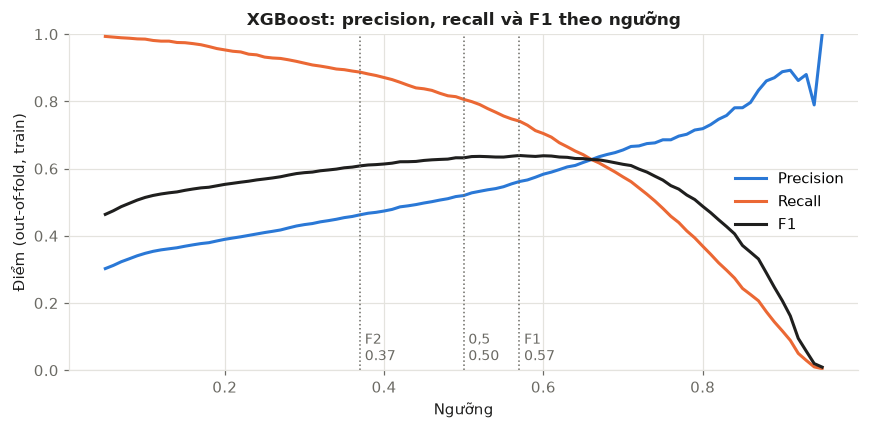
\includegraphics[width=0.8\textwidth]{img/nb_threshold_xgb.png}
\caption{Precision, Recall và F1 của XGBoost theo ngưỡng (out-of-fold trên tập train)}
\label{fig:threshold}
\end{figure}

\subsubsection{Phân tích}
\begin{itemize}
    \item \textbf{Ngưỡng tối ưu F1 cao hơn 0,5} (0,57--0,60). Class weight đã đẩy xác suất dự đoán lên cao, khiến ở ngưỡng 0,5 mô hình nghiêng hẳn về Recall (khoảng 0,80); ngưỡng tối ưu F1 kéo cân bằng ngược lại một chút về phía Precision.
    \item \textbf{Mức cải thiện F1 nhỏ} (+0,007 đến +0,008) và chỉ ở 3--4/5 fold. Đường F1 khá phẳng trong khoảng 0,45--0,65 (Hình~\ref{fig:threshold}), nên chọn ngưỡng nào trong khoảng này cũng cho F1 gần như nhau. Vai trò chính của ngưỡng là \textit{điều chỉnh cân bằng Precision--Recall} theo nhu cầu kinh doanh, không phải tăng F1.
    \item \textbf{Ngưỡng F2} (0,26--0,37) cho Recall 0,89--0,92 nhưng F1 giảm 0,02--0,05: phù hợp khi doanh nghiệp coi việc bỏ sót khách hàng rời bỏ tốn kém hơn nhiều so với gửi nhầm ưu đãi.
\end{itemize}

% ============================================================
\subsection{Kết quả cuối cùng trên tập test}\label{sec:final_test}
% ============================================================
\textbf{Chọn mô hình:} trước khi dùng tập test, nhóm chọn \textbf{XGBoost đã tuning, class weight, ngưỡng 0,57} làm mô hình chính vì có PR-AUC cross-validation cao nhất (0,671). Tập test (1.409 khách hàng, 374 rời bỏ) chỉ được dùng một lần ở bước này (\texttt{python -m src.evaluate --model-dir outputs/models/tuned}).

\begin{table}[H]
\centering
\small
\resizebox{\textwidth}{!}{%
\begin{tabular}{lcccccccc}
\toprule
\textbf{Mô hình} & \textbf{Ngưỡng} & \textbf{Precision} & \textbf{Recall} & \textbf{F1} & \textbf{F1 ở 0,5} & \textbf{ROC-AUC} & \textbf{PR-AUC} & \textbf{TP / FN / FP} \\
\midrule
\textbf{XGBoost} & 0,57 & 0,550 & \textbf{0,749} & \textbf{0,634} & 0,627 & \textbf{0,846} & \textbf{0,662} & 280 / 94 / 229 \\
Random Forest & 0,60 & \textbf{0,566} & 0,695 & 0,624 & 0,639 & 0,843 & 0,651 & 260 / 114 / 199 \\
Decision Tree & 0,60 & 0,559 & 0,719 & 0,629 & 0,627 & 0,835 & 0,624 & 269 / 105 / 212 \\
Logistic Regression & 0,60 & 0,539 & 0,706 & 0,611 & 0,614 & 0,842 & 0,633 & 264 / 110 / 226 \\
\bottomrule
\end{tabular}}
\caption{Kết quả trên tập test của các mô hình đã tuning (class weight, ngưỡng tối ưu F1)}
\label{tab:final_test}
\end{table}

\begin{figure}[H]
\centering
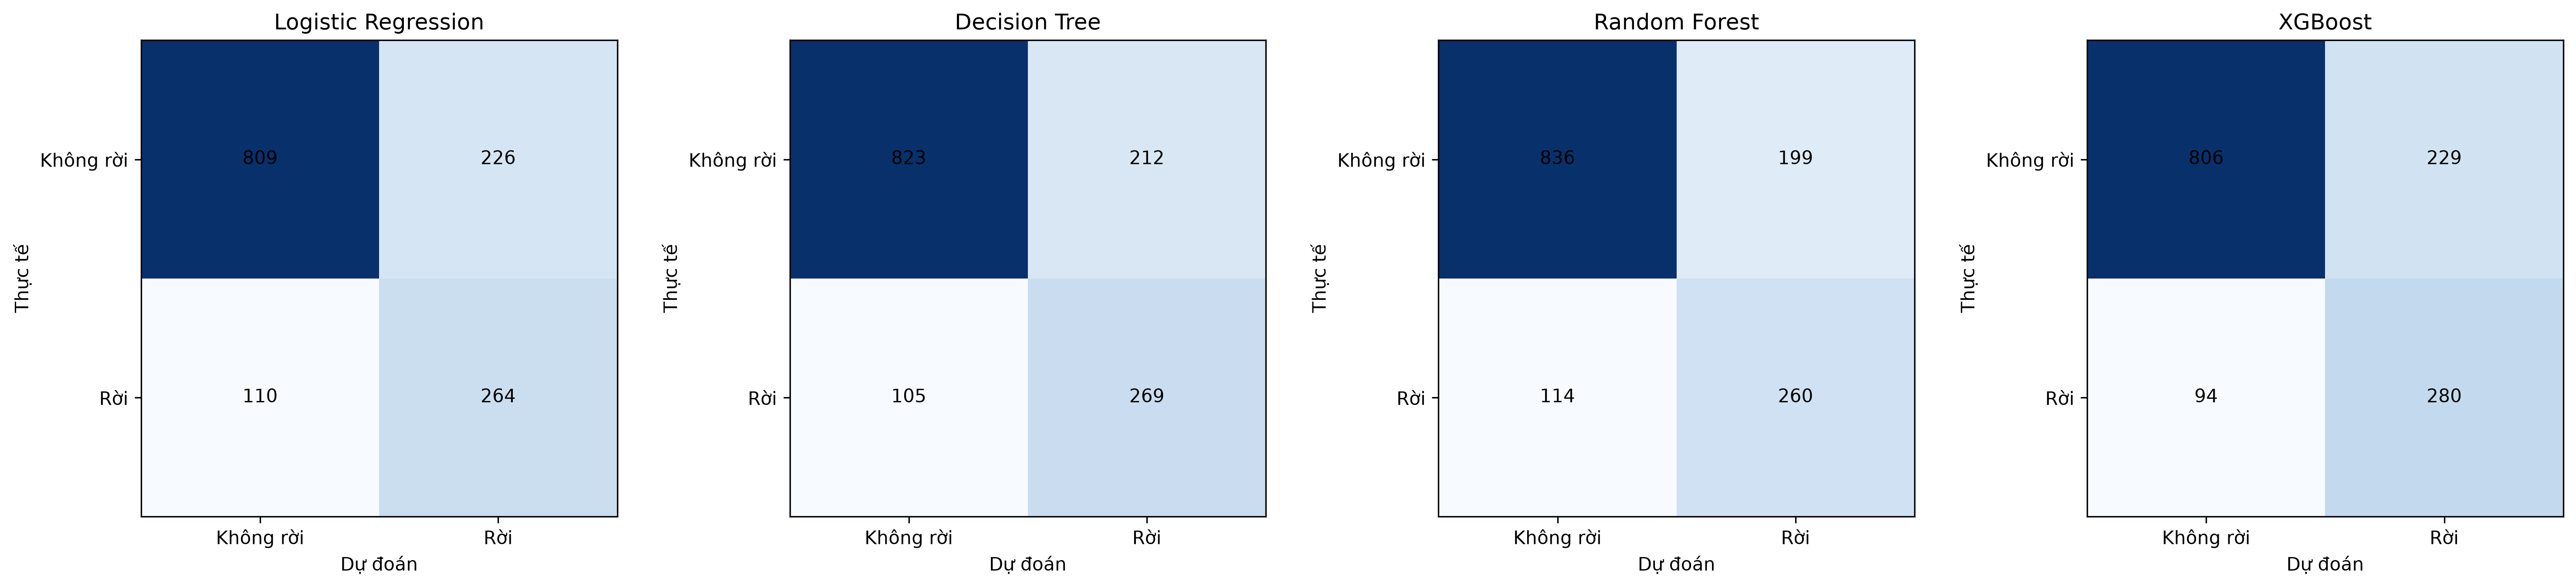
\includegraphics[width=\textwidth]{img/final_confusion.png}
\caption{Confusion Matrix trên tập test của các mô hình đã tuning với ngưỡng tối ưu F1}
\end{figure}

\begin{figure}[H]
\centering
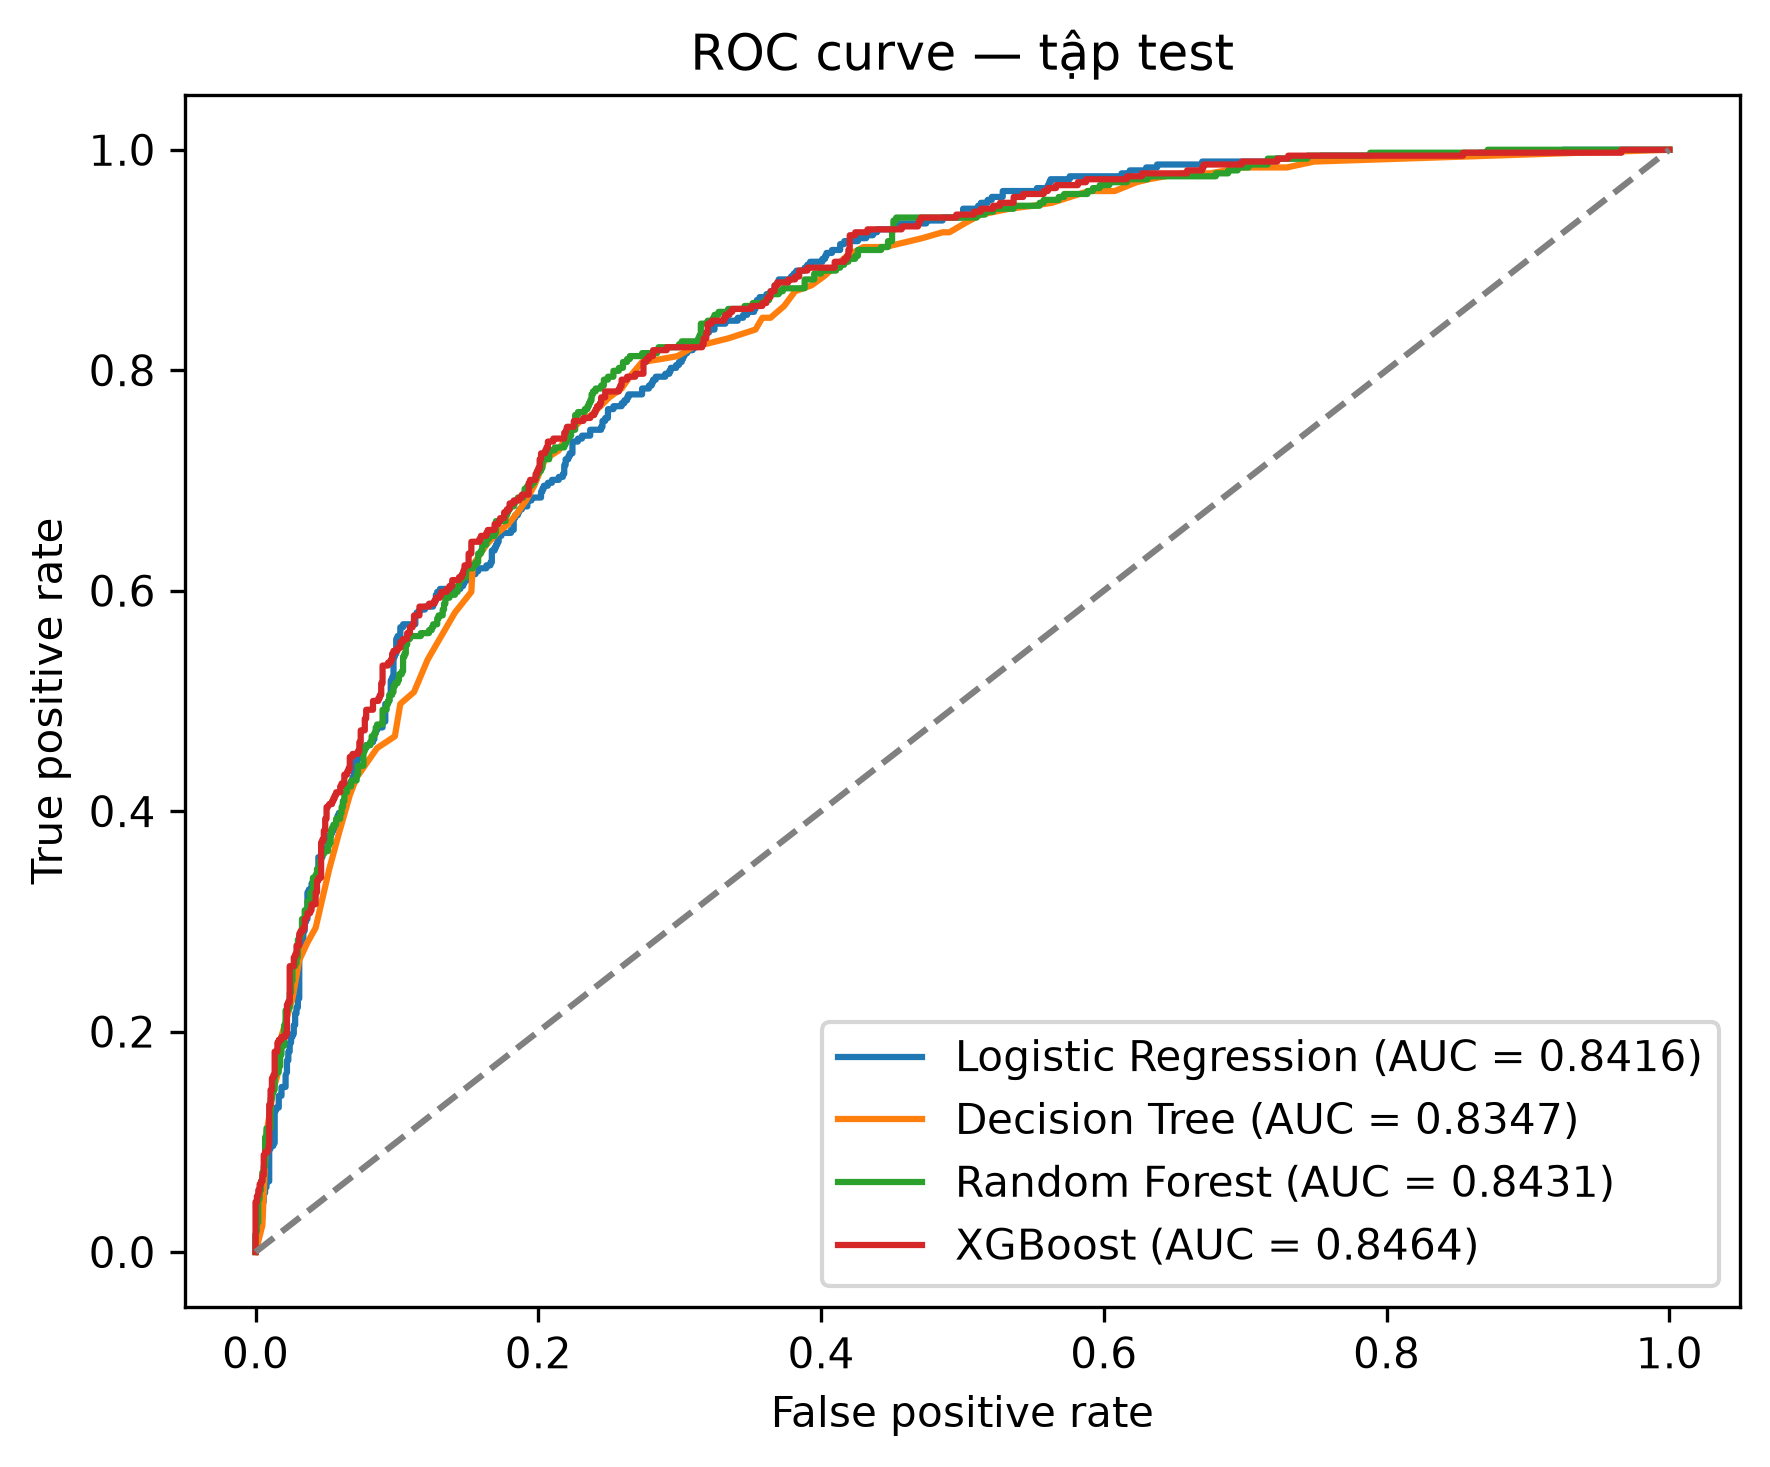
\includegraphics[width=0.49\textwidth]{img/final_roc.png}
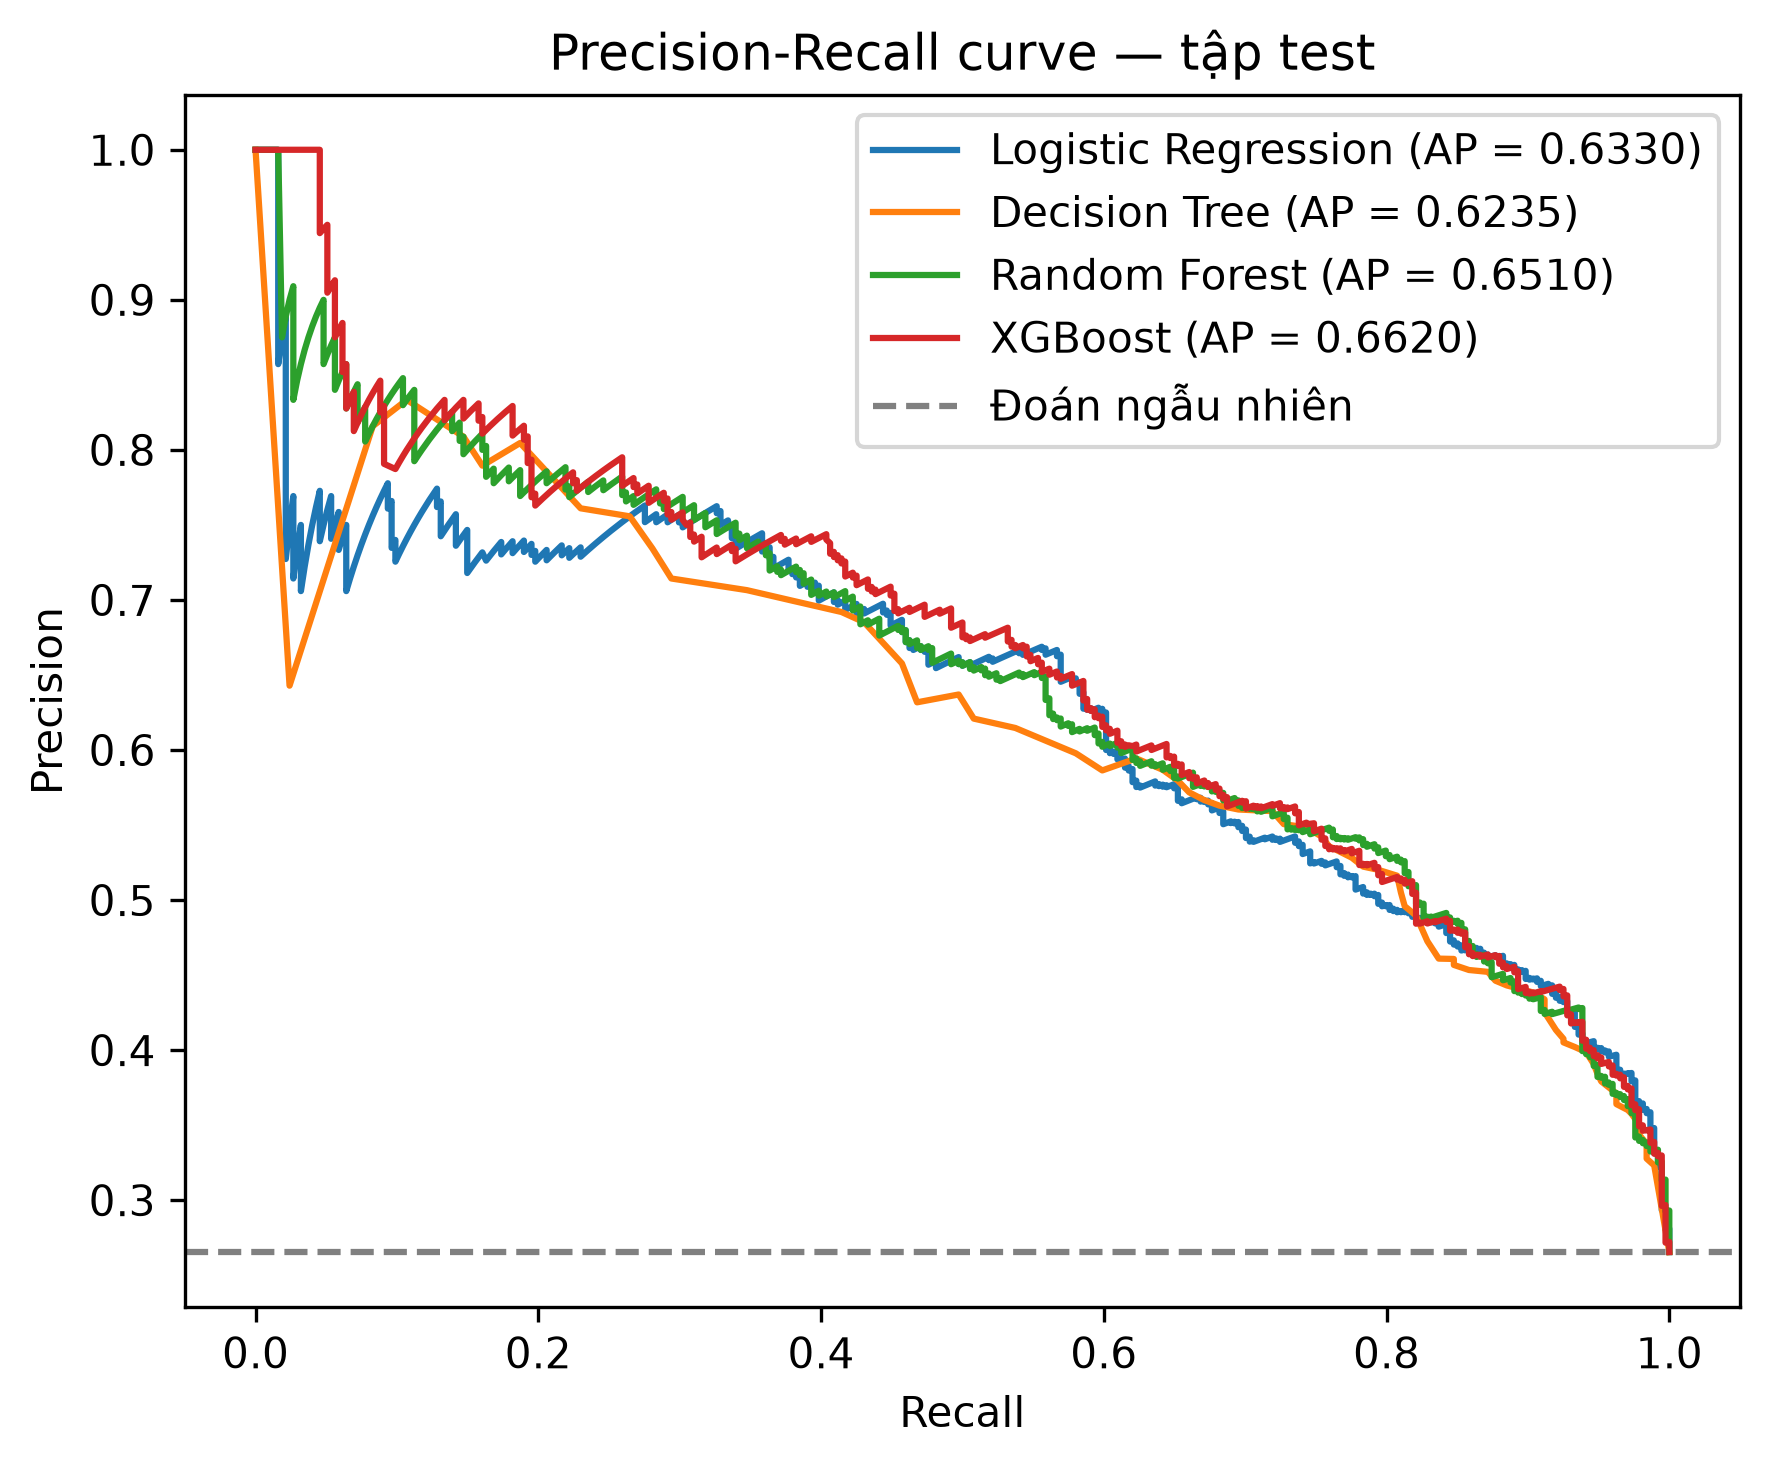
\includegraphics[width=0.49\textwidth]{img/final_pr.png}
\caption{Đường ROC (trái) và Precision--Recall (phải) trên tập test}
\end{figure}

\begin{table}[H]
\centering
\small
\resizebox{\textwidth}{!}{%
\begin{tabular}{lccccccc}
\toprule
\textbf{Mô hình} & \textbf{CV F1} & \textbf{Test F1} & \textbf{CV ROC-AUC} & \textbf{Test ROC-AUC} & \textbf{CV PR-AUC} & \textbf{Test PR-AUC} & \textbf{$\Delta$PR-AUC} \\
\midrule
Logistic Regression & 0,637 & 0,611 & 0,846 & 0,842 & 0,660 & 0,633 & $-$0,027 \\
Decision Tree & 0,628 & 0,629 & 0,830 & 0,835 & 0,630 & 0,624 & $-$0,007 \\
Random Forest & 0,639 & 0,624 & 0,848 & 0,843 & 0,667 & 0,651 & $-$0,016 \\
XGBoost & 0,639 & 0,634 & 0,850 & 0,846 & 0,671 & 0,662 & $-$0,009 \\
\bottomrule
\end{tabular}}
\caption{So sánh cross-validation và tập test (cùng ngưỡng)}
\label{tab:cv_vs_test}
\end{table}

Nhận xét:
\begin{itemize}
    \item \textbf{XGBoost đạt kết quả tốt nhất trên tập test} ở F1 (0,634), Recall (0,749), ROC-AUC (0,846) và PR-AUC (0,662), khớp với lựa chọn dựa trên cross-validation. Mô hình phát hiện được 280/374 khách hàng rời bỏ; đổi lại có 229/1.035 khách hàng ở lại bị cảnh báo nhầm.
    \item \textbf{Kết quả test khớp với cross-validation}: ROC-AUC sai khác không quá 0,005 và PR-AUC giảm 0,007--0,027 (Bảng~\ref{tab:cv_vs_test}). Mức giảm nhỏ này phản ánh độ lạc quan của việc chọn siêu tham số và ngưỡng trên cùng các fold; với XGBoost chỉ là 0,009 PR-AUC. Quy trình chọn mô hình không bị overfit vào các fold.
    \item \textbf{Chênh lệch giữa các mô hình nhỏ}: F1 của bốn mô hình nằm trong khoảng 0,611--0,634. Với 374 khách hàng rời bỏ trong tập test, chênh lệch F1 cỡ 0,02 có thể chỉ là nhiễu. Logistic Regression gần ngang bằng (ROC-AUC 0,842) và dễ giải thích hơn.
    \item \textbf{Ngưỡng tối ưu F1 trên train không đảm bảo tốt hơn 0,5 trên test}: F1 tăng với XGBoost (0,627 lên 0,634) và Decision Tree, nhưng giảm với Random Forest (0,639 xuống 0,624) và Logistic Regression. Điều này phù hợp với nhận xét ở Experiment 5 rằng đường F1 khá phẳng quanh ngưỡng tối ưu.
\end{itemize}

\textbf{Ngưỡng ưu tiên Recall (F2):} nếu dùng ngưỡng F2 (XGBoost 0,37), mô hình phát hiện 329/374 khách hàng rời bỏ (Recall 0,880) với Precision 0,460 (386 cảnh báo nhầm), F1 0,604. Đây là lựa chọn phù hợp khi chi phí của một ưu đãi thấp so với giá trị của khách hàng giữ lại được.

\textbf{So với lần đánh giá test đầu tiên} (Decision Tree và Random Forest với tham số mặc định, không xử lý mất cân bằng, ngưỡng 0,5): F1 của Decision Tree tăng từ 0,492 lên 0,629 (Recall 0,497 lên 0,719, ROC-AUC 0,654 lên 0,835); Random Forest tăng từ 0,544 lên 0,624 (Recall 0,481 lên 0,695, ROC-AUC 0,821 lên 0,843).

% ============================================================
\subsection{Giải thích mô hình}
% ============================================================

\subsubsection{Permutation importance}
Với mỗi đặc trưng gốc, nhóm xáo trộn ngẫu nhiên giá trị của nó trên tập test (20 lần) và đo mức giảm PR-AUC. Cách này áp dụng được cho mọi mô hình và làm việc trên 19 đặc trưng gốc (không phải các cột one-hot), nên dễ diễn giải.

\begin{figure}[H]
\centering
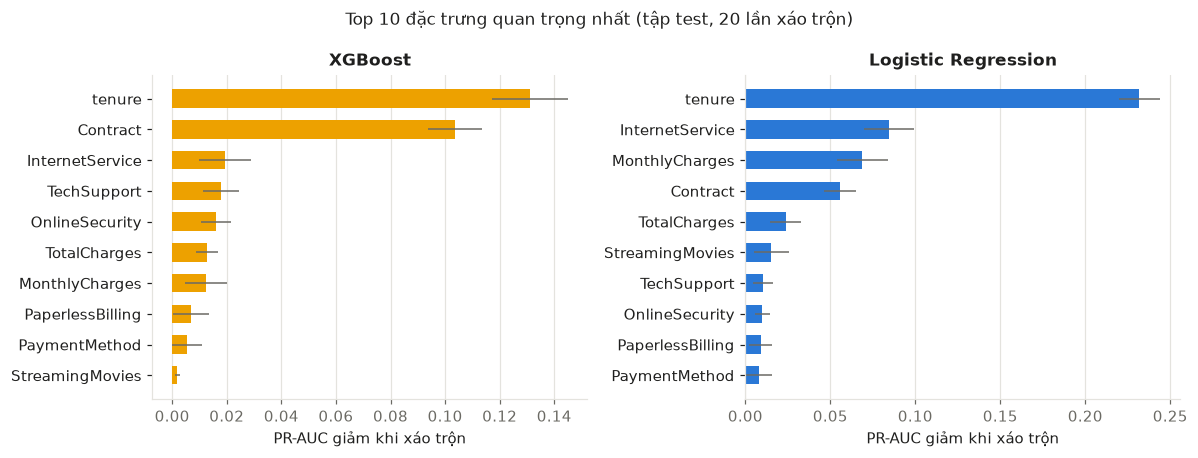
\includegraphics[width=\textwidth]{img/nb_permutation_importance.png}
\caption{Permutation importance trên tập test: mức giảm PR-AUC khi xáo trộn từng đặc trưng (10 đặc trưng quan trọng nhất; vạch: độ lệch chuẩn qua 20 lần xáo trộn)}
\label{fig:perm}
\end{figure}

\begin{table}[H]
\centering
\small
\begin{tabular}{lcc}
\toprule
\textbf{Đặc trưng} & \textbf{XGBoost} & \textbf{Logistic Regression} \\
\midrule
\texttt{tenure} & \textbf{0,131} & \textbf{0,232} \\
\texttt{Contract} & 0,104 & 0,056 \\
\texttt{InternetService} & 0,019 & 0,084 \\
\texttt{TechSupport} & 0,018 & 0,010 \\
\texttt{OnlineSecurity} & 0,016 & 0,010 \\
\texttt{TotalCharges} & 0,013 & 0,024 \\
\texttt{MonthlyCharges} & 0,012 & 0,069 \\
\texttt{PaperlessBilling} & 0,007 & 0,009 \\
\texttt{PaymentMethod} & 0,005 & 0,008 \\
\bottomrule
\end{tabular}
\caption{Mức giảm PR-AUC trên tập test khi xáo trộn từng đặc trưng}
\end{table}

\subsubsection{Hệ số Logistic Regression}
Hệ số dương làm tăng khả năng rời bỏ, hệ số âm làm giảm. Tỉ số odds $e^{\beta}$ cho biết odds rời bỏ thay đổi bao nhiêu lần khi khách hàng thuộc nhóm đó (biến one-hot) hoặc khi đặc trưng tăng một độ lệch chuẩn (biến số đã chuẩn hóa).

\begin{table}[H]
\centering
\small
\begin{tabular}{lcc@{\hskip 1.2cm}lcc}
\toprule
\multicolumn{3}{c}{\textbf{Tăng khả năng rời bỏ}} & \multicolumn{3}{c}{\textbf{Giảm khả năng rời bỏ}} \\
\cmidrule(lr){1-3} \cmidrule(lr){4-6}
\textbf{Đặc trưng} & $\beta$ & $e^{\beta}$ & \textbf{Đặc trưng} & $\beta$ & $e^{\beta}$ \\
\midrule
InternetService = Fiber optic & 0,686 & 1,98 & \texttt{tenure} & $-$1,151 & 0,32 \\
Contract = Month-to-month & 0,656 & 1,93 & Contract = Two year & $-$0,774 & 0,46 \\
\texttt{TotalCharges} & 0,484 & 1,62 & \texttt{MonthlyCharges} & $-$0,632 & 0,53 \\
StreamingMovies = Yes & 0,265 & 1,30 & InternetService = DSL & $-$0,609 & 0,54 \\
StreamingTV = Yes & 0,251 & 1,29 & InternetService = No & $-$0,268 & 0,77 \\
PaymentMethod = Electronic check & 0,240 & 1,27 & & & \\
OnlineSecurity = No & 0,199 & 1,22 & & & \\
TechSupport = No & 0,165 & 1,18 & & & \\
\bottomrule
\end{tabular}
\caption{Các hệ số lớn nhất của Logistic Regression đã tuning}
\end{table}

\subsubsection{Nhận xét}
\begin{itemize}
    \item \textbf{\texttt{tenure} là đặc trưng quan trọng nhất} với cả hai mô hình: khách hàng càng gắn bó lâu càng ít rời bỏ (mỗi độ lệch chuẩn \texttt{tenure}, khoảng 24 tháng, làm odds rời bỏ giảm còn 0,32 lần).
    \item \textbf{\texttt{Contract}} đứng thứ hai với XGBoost: hợp đồng theo tháng làm odds rời bỏ tăng gần gấp đôi, hợp đồng 2 năm làm giảm còn khoảng một nửa.
    \item \textbf{\texttt{InternetService}}: Fiber optic làm tăng nguy cơ rời bỏ, DSL làm giảm. Các \textbf{dịch vụ hỗ trợ} (\texttt{TechSupport}, \texttt{OnlineSecurity}) và \textbf{thanh toán bằng Electronic check} cũng làm tăng nguy cơ.
    \item Các đặc trưng nhân khẩu học (giới tính, có vợ/chồng, người phụ thuộc) không có mặt trong nhóm quan trọng nhất. Kết quả thống nhất với các quan sát trong phần EDA (Mục~\ref{sec:eda}).
    \item \textbf{Lưu ý về đa cộng tuyến:} \texttt{TotalCharges} xấp xỉ \texttt{tenure} $\times$ \texttt{MonthlyCharges}, nên ba biến này tương quan mạnh với nhau. Dấu hệ số của từng biến riêng lẻ (\texttt{MonthlyCharges} âm, \texttt{TotalCharges} dương) không nên diễn giải tách rời. Permutation importance đáng tin cậy hơn để đánh giá mức độ quan trọng, nhưng cũng có thể đánh giá thấp các đặc trưng tương quan với nhau. Các giải thích này là quan hệ thống kê mà mô hình học được, không phải quan hệ nhân quả.
\end{itemize}

% ============================================================
\subsection{Tổng hợp kết quả}
% ============================================================

\begin{figure}[H]
\centering
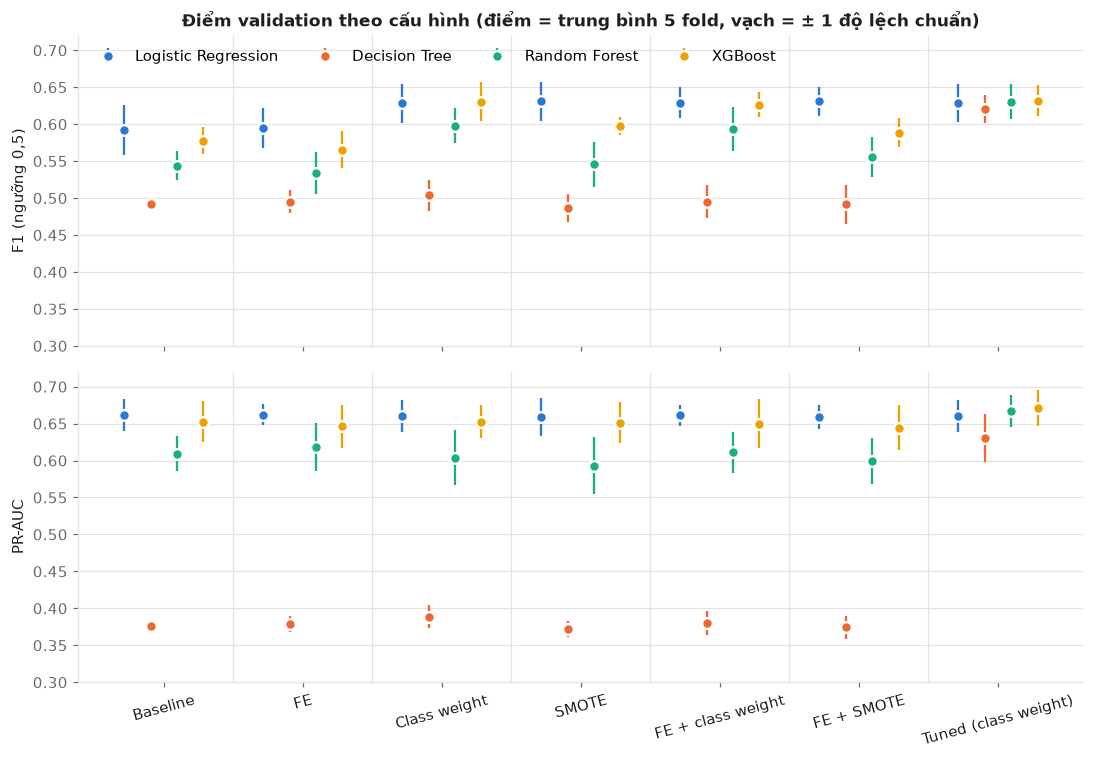
\includegraphics[width=\textwidth]{img/nb_cv_overview.png}
\caption{F1 (ngưỡng 0,5) và PR-AUC validation của mọi cấu hình (chấm: trung bình 5 fold; vạch: $\pm$ 1 độ lệch chuẩn)}
\label{fig:cv_overview}
\end{figure}

\begin{table}[H]
\centering
\small
\begin{tabular}{l c p{9cm}}
\toprule
\textbf{Thay đổi} & \textbf{Tác động} & \textbf{Ghi chú} \\
\midrule
Class weight & \textbf{Lớn} & F1 +0,036 đến +0,054 với LR, RF, XGBoost (5/5 fold); Recall tăng 0,16--0,26; đổi lại Precision giảm. \\
SMOTE & Trung bình & Tương đương class weight với LR; yếu hơn với mô hình cây. Class weight đơn giản hơn và không sinh dữ liệu giả. \\
Tuning & \textbf{Lớn với mô hình cây} & Decision Tree: F1 +0,12, PR-AUC +0,24; Random Forest: F1 +0,03, PR-AUC +0,06; nhờ giới hạn độ sâu và kích thước lá, giảm overfit. Không đổi với LR. \\
Feature Engineering & Không đáng kể & Mọi chênh lệch trong khoảng $\pm 0{,}012$, nhỏ hơn độ dao động giữa các fold. \\
Chọn ngưỡng & Nhỏ với F1 & +0,008 F1 trên CV, trên test lúc tăng lúc giảm. Chủ yếu dùng để điều chỉnh cân bằng Precision--Recall. \\
\bottomrule
\end{tabular}
\caption{Tác động của từng kỹ thuật}
\label{tab:summary_effects}
\end{table}

Hình~\ref{fig:cv_overview} và Bảng~\ref{tab:summary_effects} cho thấy hai kỹ thuật mang lại cải thiện chính là \textbf{xử lý mất cân bằng bằng class weight} (giải quyết Recall thấp) và \textbf{tuning} (giải quyết overfitting của mô hình cây). Sau khi kết hợp hai kỹ thuật này, bốn mô hình đạt hiệu năng rất sát nhau, cho thấy giới hạn hiện tại nằm ở thông tin có trong dữ liệu hơn là ở lựa chọn thuật toán.
